\documentclass{book}
\usepackage{graphicx} % Required for inserting images
\usepackage{subcaption}

\usepackage[utf8]{inputenc}
\usepackage[T1]{fontenc}
\usepackage{listings}
\usepackage{appendix}
\usepackage{siunitx}
\usepackage{multirow}
\usepackage[version=4]{mhchem}
\usepackage{natbib}
\usepackage{booktabs}
\usepackage{bachelorstitlepageUNAM}
\usepackage[spanish,es-nodecimaldot,es-tabla]{babel}
\usepackage{tikz} 
\usepackage{tocloft}
\graphicspath{{./figs/}}
\usepackage{setspace}
\usepackage{hyperref}
\usepackage{float}              % Para usar [H] en las figures

\usepackage{tikz}
\usepackage{lipsum}
\usepackage{caption}

\DeclareSIUnit\msun{\text{M\ensuremath{_\odot}}}
\usepackage{astrojournals}
\bibliographystyle{aasjournal}
\renewcommand{\lstlistingname}{Algoritmus}

\title{Avances de tesis}
\author{r.reyes }
\date{December 2023}

\begin{document}

    \begin{titlepage}
        \thispagestyle{empty}
        \begin{minipage}[c][0.17\textheight][c]{0.25\textwidth}
            \begin{center}
                \includegraphics[width=3.5cm, height=3.5cm]{Escudo-UNAM.pdf}
            \end{center}
        \end{minipage}
        \begin{minipage}[c][0.195\textheight][t]{0.75\textwidth}
            \begin{center}
                \vspace{0.3cm}
                \textsc{\large Universidad Nacional Aut\'onoma de M\'exico}\\[0.5cm]
                \vspace{0.3cm}
                \hrule height2.5pt
                \vspace{.2cm}
                \hrule height1pt
                \vspace{.8cm}
                \textsc{Instituto de Radioastronomía y astrofísica}\\[0.5cm] %
            \end{center}
        \end{minipage}

        \begin{minipage}[c][0.81\textheight][t]{0.25\textwidth}
            \vspace*{5mm}
            \begin{center}
                \hskip2.0mm
                \vrule width1pt height13cm 
                \vspace{5mm}
                \hskip2pt
                \vrule width2.5pt height13cm
                \hskip2mm
                \vrule width1pt height13cm \\
                \vspace{5mm}
                \includegraphics[height=4.0cm]{logoIRyAnegro_1.png}
            \end{center}
        \end{minipage}
        \begin{minipage}[c][0.81\textheight][t]{0.75\textwidth}
            \begin{center}
                \vspace{1cm}

                {\large\scshape El impacto del viento estelar y la radiación en glóbulos neutros alrededor de una estrella Wolf-Rayet}\\[.2in]

                \vspace{2cm}            

                \textsc{\LARGE T\hspace{1.5cm}E\hspace{1.5cm}S\hspace{1.5cm}I\hspace{1.5cm}S}\\[0.5cm]
                \textsc{\large que para obtener el grado de:}\\[0.5cm]
                \textsc{\large Maestro en ciencias (astrofísica)}\\[0.5cm]
                \textsc{\large presenta:}\\[0.5cm]
                \textsc{\large {Roberto Reyes Cabañas}}\\[2cm]          

                \vspace{0.5cm}

                {\large\scshape Tutor:\\[0.3cm] {Dr. William John Henney }}\\ [.2in]

                \vspace{0.5cm}

                \large{Morelia, Michoacán,}{ }{2024}
            \end{center}
        \end{minipage}
    \end{titlepage}

%\maketitle

\chapter*{Resumen}

La nebulosa circunestelar M1-67 alrededor de la estrella Wolf-Rayet WR~124 contiene cientos de pequeños glóbulos neutros, como revelan imágenes recientes del JWST. La emisión ionizada de la nebulosa muestra un patrón intrincado de cáscaras y filamentos, muchos de los cuales parecen asociados con los glóbulos pero desplazados hacia la estrella central. Proponemos un modelo simple para la nebulosa en el que los flujos de fotoevaporación desde la superficie irradiada de los glóbulos interactúan con el viento estelar de la estrella Wolf-Rayet para formar cáscaras de emisión hemisféricas. Probamos este modelo contra imágenes del JWST y H alpha del HST de la nebulosa, encontrando una buena concordancia para los glóbulos mejor observados y más aislados. El modelo proporciona una explicación física para la morfología observada de la nebulosa y los glóbulos, y sugiere que los glóbulos están protegidos hidrodinámicamente del viento estelar por los flujos de fotoevaporación. Derivamos una estimación independiente de la fuerza del viento estelar, que es consistente con valores previamente derivados de la modelación de la atmósfera estelar. También somos capaces de restringir la distribución tridimensional de los glóbulos.

\newpage

\tableofcontents

\newpage

\chapter{Introducción}

Los \textit{glóbulos} son concentraciones densas de gas y polvo en el medio interestelar que se cree que se forman por inestabilidades térmicas, colapso gravitacional o turbulencia. Estos glóbulos se pueden formar en regiones de formación estelar masiva o en nebulosas alrededor de estrellas evolucionadas.

En general los glóbulos tienen una gran variedad de tamaños. Por ejemplo, cuando nos referimos a los glóbulos en regiones de formación estelar masiva comúnmente suelen ser de gran tamaño, $\sim$\SI{0.1}{pc}, mientras que en nebulosas alrededor de estrellas evolucionadas son de un tamaño más pequeño, $\sim$\SI{e-2}{pc}.

Los primeros glóbulos fueron observados por Bart Bok en 1940. Como podemos ver en la figura \ref{fig:Banard}, debido a a que las estrellas de fondo sufren enrojecimiento por polvo, estos glóbulos se pueden apreciar como nubes oscuras ya que tienen gran cantidad de gas neutro y polvo. Los glóbulos contienen principalmente hidrógeno molecular en su interior, así como también pueden tener otras moléculas, metales e incluso algunos silicatos. Si bien puede haber formación estelar en su interior no podemos ver la radiación de las estrellas ya que es absorbida por el hidrógeno atómico y el polvo, es por eso que se ven oscuras.

Cuando los glóbulos se encuentra en regiones de formación estelar masiva, estos pueden interactuar con la radiación ultravioleta (UV) de las estrellas jóvenes masivas que se encuentren cerca, o con la de la estrella central en el caso de que los glóbulos estén en una nebulosa circunestelar. En estos casos se puede observar el frente de ionización como un borde brillante de emisión.

\begin{figure}[htb]
    \centering
    \includegraphics[width=0.85\textwidth]{images Chapter 1/C1_Bok_globule.jpg}
    \caption{Ejemplo de un glóbulo de Bok. Imagen de Banard 68 visto con Very Large Telescope FORS1 en 440 nm, 557 nm y 768 nm. Se puede apreciar una zona oscura el cual es el glóbulo y lo que pareciera ser enrojecimiento de las estrellas por polvo en la superficie del glóbulo. En esta imagen podemos ver que no hay evidencia de alguna fotoevaporación externa por parte de estrellas. \citep{Alves:2001}.}
    \label{fig:Banard}
\end{figure}

Esta interacción entre estrellas y glóbulos se puede dar a diferentes escalas, lo que nos da una gran variedad de estructuras. Entre las de mayor tamaño se encuentran lo que parecen ser columnas, pilares o trompas de elefantes, como se les conoce en la literatura, que llegan a tener un tamaño de $\sim$\SI{1}{pc} y una densidad del orden de \SI{e3}{cm^{-3}}. Esta interacciones también se puede dar dentro de regiones HII, como vemos en la figura \ref{fig:Pillars}.

\begin{figure}[htb]
    \centering
    \includegraphics[width=1 \textwidth]{images Chapter 1/C1_Pillars.jpg}
    \caption{En \textbf{A} vemos dos ejemplos de pilares, donde la imagen derecha de cada ejemplo es vista a \SI{2.12}{\mu m} (\SI{}{H_2}) y la imagen izquierda es \SI{}{H_2-Br_{\gamma}} \citep{Hartigan:2015}. \textbf{B} es un ejemplo de una trompa de elefante, es una imagen de M16 tomada con WFPC2 con e filtro F656N, los \SI{30}{\arcsecond} corresponden \SI{9e17}{cm} (\SI{0.29}{pc}) \citep{JJHester:1996}. \textbf{C} es el outflow de Tadpole globule, el cual consta del sistema HH900 jet+outflow, la imagen de abajo es vista en \SI{}{H_\alpha} con el continuo 
    \citep{MeganReiter:2019}. }
    \label{fig:Pillars}
\end{figure}

En escalas más pequeñas están lo que se conoce como EGGs (Evaporating Gaseous Globule) los cuales tienen tamaños de $\sim$\SI{e-2}{pc}, y los proplyds que tienen tamaños $\le\SI{e-2}{pc}$. 


Estos glóbulos no solo se encuentran en regiones de formación estelar, también hay dentro de nebulosas alrededor de estrellas evolucionadas donde se les conoce más comúnmente como \textit{nudos}, un ejemplo de esto es la imagen \textbf{D} de la figura \ref{fig:nudos}. En este trabajo estudiaremos más a fondo los nudos que hay en una nebulosa alrededor de cierta estrella evolucionada.

\begin{figure}[htb]
    \centering
    \includegraphics[width=1 \textwidth]{images Chapter 1/C1_Globulettes.jpg}
    \caption{En \textbf{A} vemos proplyds con su bowshock en Orion tomado con HST planetary camera, la barra negra indica una medida de \SI{1}{\arcsecond} que corresponde a 430 AU (\SI{2e-3}{pc}) \citep{Garcia-Arredondo:2001}. \textbf{B} son ejemplos de EGGs en Carina, tomado con WFC3, ACS, WFPC2 \citep{Mesa-Delgado:2016}. \textbf{C} es el globulette denso RN88 visto en \SI{}{H_\alpha} con un diámetro de \SI{6}{\arcsecond} (\SI{4e-2}{pc}) en la nebulosa de Rosette \citep{GFGahm:2013}. \textbf{D} son ejemplos de nudos en la nebulosa de la Hélice, los mosaicos tienen una medida de \SI{47.5}{\arcsecond}$\times$\SI{44.8}{\arcsecond} (\SI{4.76e-2}{pc}$\times$\SI{4.49e-2}{pc}) \citep{O'Dell:2007}. }
    \label{fig:nudos}
\end{figure}



\section{Flujos de fotoevaporación ionizada} \label{Sec:fluijos fotoevaporativos}

Todos los ejemplos de las figuras \ref{fig:Banard}, \ref{fig:Pillars} y \ref{fig:nudos} se encuentran ya sea en regiones de formación estelar o en nebulosas alrededor de estrellas evolucionadas. 

Lo interesante en todos estos ejemplos es la forma que toman al interaccionar con las estrellas más masivas que se encuentran cerca, esto para los glóbulos que se encuentran en regiones de formación estelar.  Mientras que los que se encuentran en nebulosas planetarias interactúan con la estrella evolucionada. Durante estas interacciones en algunos casos podemos ver lo que se conoce como \textit{flujos fotoevaporativos}, los cuales explicaremos mejor a continuación.

En el caso de las regiones de formación estelar podemos considerar una estrella masiva y una nube densa de gas neutro. En esta interacción es necesario que la estrella sea masiva, o que tenga un gran flujo ionizante como para poder ionizar el gas neutro, de lo contrario no podremos ver el flujo fotoevaporativo. Recordemos que en las regiones de formación estelar hay muchas estrellas nuevas que emiten principalmente en radio o infrarrojo, por lo que no todas las estrellas nuevas pueden ionizar el gas neutro.

\cite{OortySpitzer_1955} explican de manera detallada como es la interacción entre una estrella tipo O y una nube interestelar de gas neutro. Con esto podemos explicar de una mejor manera como es la interacción en regiones de formación estelar masiva. Ellos consideran tres partes importantes para esto: La estrella ionizante, la nube interestelar de gas neutro y la región que hay entre la estrella y la nube interestelar. La nube interestelar debe ser mucho más densa y fría que la región que hay entre la estrella y la nube como vemos en la figura \ref{kahn_zones}.

\begin{figure}[htb]
    \centering
    \includegraphics[width= \textwidth]{artesanales/ImgFi01-5.pdf}
    \caption{Esquema inicial utilizado en \cite{Kahn:1954}}
    \label{kahn_zones}
\end{figure}

Cuando la radiación UV comienza a calentar el gas de la nube, el gas ionizado comienza a expandirse en dirección a la estrella, esto ya que en esta dirección la densidad es menor que la de la nube y puede expandirse libremente. 

En un inicio esta radiación ioniza el gas a una tasa muy rápida causando una ``tormenta de partículas ionizantes'' que viene por parte de la nube, conforme esto va evolucionando se crea una capa aislante alrededor de la nube. Esta radiación produce un choque ionizante lo cual provoca que la nube se comprima. También se produce un frente de ionización que avanza hacia la nube haciendo que esta se vaya alejando de la estrella. Mientras esto ocurre hay un choque interno que va viajando a través de la nube a la parte trasera \citep{Bertoldi_1989}. Para que esto ocurra \cite{Kahn:1954} da cierto criterios, en los cuales dice que la radiación no debe ser muy débil o demasiado fuerte.

\section{Estrellas Wolf-Rayet y sus vientos}

Las estrellas WR (Wolf-Rayet) son estrellas evolucionadas de estrellas masivas, como estrellas tipo O, que tienen una alta pérdida de mas debido a sus grandes vientos y fueron nombradas así después de que Charles Wolf y Georges Rayet identificaran 3 estrellas en Cygnus con sus  anchas líneas de emisión que las caracterizan muy bien. 

Estas estrellas se caracterizan principalmente por sus fuertes vientos que pueden ser del orden de $\sim$\SI{1000}{km/s}, los cuales provocan sus líneas de emisión anchas. Así como también tienen una alta pérdida de masa $\sim$2--\SI{10e-5}{\msun/yr}. Típicamente son estrellas de 10--\SI{25}{\msun} que son descendientes de estrellas tipo O y se caracterizan por tener intensas líneas de emisión de libre-libre desde el $\mu$m hasta el cm \citep{crowther:2007}.

A estas estrellas se les clasifica por el cociente que hay entre sus líneas de emisión intensa que las caracterizan. \cite{Smith:1968} las clasifica principalmente como WN a aquellas que son abundantes en He y N, WC a las que son abundantes en He y C. Además les pone un número para identificar esencialmente si son tipo tardío o temprano.

\begin{table}[h]
    \begin{center}
        \begin{tabular}{c c}
        \toprule
        \multicolumn{2}{c}{Clasificación de estrellas WR} \\ \midrule
        Índice espectral    & Tipo de estrellas\\ \midrule
        WN2--5     & Tipo temprana, WNE (Early WN)\\
        WN7--9 & Tipo tardía, WNL (Late WN) \\
        WC4--6 & WCE\\
        WC7--9 & WCL \\ \bottomrule
        \end{tabular}
    \caption{Principal clasificación de estrellas WR  según sus líneas de emisión. Dentro de las WC, las que se clasifican como WC6 pueden ser de tipo tardía o temprana.}
    \label{tab:WR-clasificacion}
    \end{center}
\end{table}

También están las estrellas WO que son abundantes en He y O, pero en realidad son una extensión de las WCE. Para las estrellas en las que detectamos una cantidad considerable de H en su atmósfera se les pone también una ``h'' \citep{SSM:1996}.

Debido a que no se han encontrado muchas estrellas WR se les suele asociar un número pero este número no tiene nada que ver con su índice espectral.

\section{Estructura de la tesis}

En esta tesis proponemos un modelo simple para explicar como interactúa el flujo fotoevaporativo transónico de un glóbulo con una presión externa. Este modelo lo vamos a aplicar  a los nudos que se encuentran en la nebulosa M1-67, por lo que se explicará la interacción del flujo fotoevaporativo con la presión RAM del viento estelar de la estrella WR-124.

En el capítulo 2 vamos a hablar de cómo la interacción entre estos dos flujos supoersónicos producen cáscaras chocada, y cómo es que comparamos la presión de una cáscara chocada con un presión externa. 

\chapter{Modelos analíticos de flujos fotoevaporativos interactuando con una presión externa}
\chaptermark{Modelo analítico}\label{Chapter : Modelo}

En este capítulo vamos a describir el modelo que se propone para explicar la interacción que hay entre el flujo fotoevaporativo de un glóbulo y una presión externa. Este modelo en principio se puede aplicar a cualquier tipo de glóbulo como los que se mencionaron antes. 

En este trabajo en especial vamos a tratar en específico la interacción del flujo fotoevaporativo de los glóbulos\footnote{Llamaremos glóbulos a los nudos que hay en la nebulosa por simplicidad.} en la nebulosa M1-67 y la presión RAM por parte del viento estelar de la estrella WR-124. La presencia de estos glóbulos en la nebulosa se puede apreciar mejor en la figura \ref{fig:nudos WR124}.

Para esto hemos considerado que ya han pasado todas las fases mencionadas en la sección \ref{Sec:fluijos fotoevaporativos} y ahora estamos en un equilibrio de ionización. La forma del glóbulo en este modelo será esférico por simplicidad (Ver Apéndice \ref{App:fuerzas}).

En esta interacción entre el flujo fotoevaporativo y el viento estelar, los cuales son supersónicos, se producen dos zonas chocadas y entre estas dos zonas una discontinuidad de contacto como se describe en la figura \ref{fig:zones}. De estas zonas esperamos ver solo el flujo fotoevaporativo chocado y no el viento estelar chocado ya que este último es menos denso además de que es no radiativo y la longitud de enfriamiento es más grande que la región de interacción.

\begin{figure}[htb]
    \centering    \includegraphics[width=\textwidth]{Nuevas imagenes finales/C2_zone_new.pdf}
    \caption{La interacción entre el flujo fotoevaporativo y el viento estelar de una estrella forma 4 zonas. La línea punteada que une el centro del  glóbulo con el centro de la estrella es el eje de simetría que vamos a considerar en el modelo, vemos como en esta línea tanto el viento estelar como la radicación inciden de forma perpendicular a la base del glóbulo y en dirección contraria viaja el flujo fotoevaporativo. La zona 1 es donde el flujo fotoevaporativo sale de la superficie del glóbulo con un número de Mach igual a 1 y va aumentando. La zona 2 es el flujo fotoevaporativo chocado, la cual esperamos ver en las observaciones como una cáscara y nos vamos a referir a ella como la cáscara chocada. La zona 3 es el viento estelar chocado y la zona 4 es donde viaja el viento estelar supersónico, el cual es menos denso que el flujo fotoevaporativo. La discontinuidad de contacto se da entre las zonas 2 y 3, la línea gris.}
    \label{fig:zones}
\end{figure}

\begin{figure}[htb]
    \centering    \includegraphics[width=0.8\textwidth]{images Chapter 2/C2_Canto.jpg}
    \caption{Interacción de dos flujos supersónicos las cuales son producidas por dos fuentes (puntos negro en el eje z) a una distancia D. En esta interacción se produce una cáscara delgada R$(\theta)$ cuando los flujos llegan a un equilibrio. Para este problema se considera simetría cilíndrica \citep{Canto:1996}.}
    \label{fig:Canto1}
\end{figure}

\begin{figure}[htb]
    \centering    \includegraphics[width=\textwidth]{artesanales/ImgFi01-2.pdf}
    \caption{La radiación y el viento estelar viajan hacia el glóbulo como lo indican las flechas azules y vemos que inciden de manera perpendicular a la superficie del glóbulo en el eje de simetría. Mientras que el flujo fotoevaporativo por parte del glóbulo viaja como lo indican las flechas rojas, y por lo tanto en la interacción entre este flujo fotoevaporativo y el viento estelar debemos considerar cierto ángulo si no estamos en el eje de simetría.}
    \label{fig:cilindross}
\end{figure}

\cite{Canto:1996} trata de una manera formal la interacción entre dos flujos supersónicos en la cual considera dos fuentes separadas a una distancia D como en la figura \ref{fig:Canto1}. Cuando estos flujos que están interaccionando llegan a un equilibrio de presiones se forma una cáscara delgada.

%\begin{figure}[h]
%    \centering    \includegraphics[width=0.75\textwidth]{images Chapter 2/Chp2_cilinders.jpg}
 %   \caption{Si consideramos una simetría cilíndrica con un radio muy pequeño, podemos tratar este problema de manera radial y de tal manera que la radiación y el viento estelar inciden de manera perpendicular al glóbulo.}
 %   \label{fig:cilinders}
%\end{figure}

\section{Modelo hidrodinámico estacionario}

Para este modelo es importante mencionar que no estamos considerando ninguna fuerza de gravedad por parte de la estrella o del mismo glóbulo, así como tampoco ninguna otra fuerza externa. De igual manera, no vamos a considerar campos magnéticos por simplicidad.

Para este trabajo en particular solo vamos a considerar como presión externa la presión RAM del viento estelar por parte de la estrella WR-124.

Tomando en cuenta que el tiempo en el que ocurren las fases mencionadas en la sección \ref{Sec:fluijos fotoevaporativos} es muy corto comparado con el tiempo de interacción que hay entre el flujo fotoevaporativo y el viento estelar, vamos a suponer que la capa aislante producida por la radicación UV ya se ha formado y ahora estamos en equilibrio de ionización. Por lo que vamos a considerar este modelo como estacionario, es decir, que los tamaños del glóbulo y de la cáscara chocada los vamos a tomar como constantes ya que no cambiaran sus tamaños de manera significativa.

En la figura \ref{fig:cilindross} vemos que podemos simplificar este problema si ponemos un cilindro de radio pequeño alrededor del eje de simetría.  En este cilindro podemos ignorar los movimientos transversales ya que los gradientes en estas direcciones son muy pequeños si los comparamos con los gradientes en la dirección axial. 

Alrededor del eje de simetría podemos ver como tanto la radiación UV y el viento estelar inciden de manera perpendicular a la base del glóbulo y viajan en dirección contraria el flujo fotoevaporativo por parte del glóbulo. Por lo que primero vamos a resolver este problema solo en el eje de simetría, ya que aquí se vuelve unidimensional. Más adelante vamos a considerar qué pasaría si resolvemos este problema considerando un ángulo $\theta$ con respecto al eje de simetría.

% Balance between ionizations and recombinations

\section{Ecuación de estado y equilibrio de ionización}

Para este caso vamos a considerar que el gas que esta interaccionando con el viento estelar de la estrella es un gas ideal, por lo que nuestra ecuación de estado será
\begin{equation}
    PV = Nk_BT
\end{equation} 
donde $P$ es la presión del gas, $V$ su volumen, $N$ es el número de partículas, $k_B$ la constante de Boltzman y $T$ es la temperatura. De aquí tenemos que \begin{equation}
    P = nk_BT = \frac{\rho k_B T}{\bar{m}}
\end{equation}
donde $n$ es la densidad numérica, $\rho$ la densidad de masa y $\bar{m}$ es la masa promedio. En este caso estamos considerando que el gas contiene principalmente hidrógeno y una pequeña fracción de helio, por lo que vamos a considerar una masa promedio de \SI{0.6}{m_{p}} en el gas ionizado.

En este gas ideal vamos a tomar la velocidad del sonido isotérmica, la cual está dada por
\begin{equation}
    c_s  = \sqrt{\frac{k_B T}{\bar{m}}}
\end{equation} 
de esta manera vemos que la velocidad del sonido en el gas ionizado solo depende de su temperatura. En este tipo de gases la velocidad del sonido es típicamente del orden de \SI{e6}{cm.s^{-1}}

En este modelo vamos a considerar que  ya ha sucedido la tormenta de partículas ionizantes, la fase de implosión y se ha formado la capa aislante como se mencionó en la sección \ref{Sec:fluijos fotoevaporativos}, por lo que vamos a considerar que el flujo de fotones ionizantes por unidad de tiempo por parte de la estrella ionizante 
\begin{equation}
    S_* = \int_{\nu_0}^\infty \frac{L_\nu}{h\nu}d\nu
\end{equation} 
donde $L_\nu$ es la luminosidad de la estrella por unidad de frecuencia y $\nu_0$ es la frecuencia a la que los fotones tienen energía de \SI{13.6}{eV}, esta en equilibrio con la tasa total de recombinaciones que esta dada por 
\[n_e n_i h \alpha_\mathrm{B}\] 
donde $\alpha_\mathrm{B}$ es el coeficiente de recombinación para el caso B. Este coeficiente de recombinación para el caso B toma en cuenta las recombinaciones a todos los niveles, excepto al nivel base, esto ya que el fotón liberado en esta recombinación al nivel base puede volver a ionizar algún otro átomo que se encuentre muy cerca. 

\section{Estructura del flujo fotoevaporativo}\label{Estructura}

En este modelo  estamos considerando un frente D-crítico para el frente de ionización \citep{Shuu:1992}, esto es, que en la parte neutra tenemos una expansión subsónica y hay un punto sónico interior al frente de ionización a partir del cual tendremos una expansión supersónica en la zona ionizada. En este caso por simplicidad vamos a considerar el frente de ionización como una discontinuidad en el que pasamos de tener gas no ionizado a tener un gas totalmente ionizado, por lo que tomaremos que el punto sónico se da justo en $r_0$. Así que vamos a considerar que el gas tiene un número de Mach igual a 1 en $r_0$ y este va a ir aumentando conforme atraviesa toda la zona 1 de la figura \ref{fig:zones} ya que se va expandiendo libremente. En principio podríamos tomar que tanto el radio del glóbulo como la densidad en su superficie son parámetros libres, pero con las observaciones podemos medir el radio y la densidad la podemos calcular ya que esta debe ser consistente por haber considerado equilibrio de ionización.

Con este modelo se pretende ver hasta donde llegamos a un equilibrio de presión entre la presión por parte del flujo fotoevaporativo y la presión RAM del viento estelar. Para el caso de la presión del flujo fotoevaporativo vamos a considerar tanto la presión térmica como la hidrodinámica, por lo que la presión total en la base del glóbulo está dada por
\begin{equation}\label{eq: Presion total}
    P_{tot}=P_{ter}+P_{hid}=n\bar{m}c_s^2+n\bar{m}u^2=\rho c_s^2(1+M^2)
\end{equation}
En este caso, como ya habíamos mencionado antes, no estamos considerando presión magnética ni de radiación.

\begin{figure}[htb]
    \centering \includegraphics[width=\textwidth]{artesanales/ImgFi01-3.pdf}
    \caption{$r_0$ es el radio del glóbulo, la parte neutra, mientras que $\rho_0,M_0$ y $P_0$ son los valores que tenemos en la superficie del glóbulo y conforme estos avanzan con dirección a la estrella sus valores van cambiando hasta tener diferentes valores en $r_1$, que es el radio del centro del glóbulo hasta la base del flujo fotoevaporativo chocado, $\rho,M$ y $P$ son los valores que tendrán en la base del flujo fotoevaporativo chocado.}
    \label{fig:parameters}
\end{figure}

Este equilibrio de presión se logrará a un radio $r_1$ que es donde la presión del flujo fotoevaporativo ha disminuido un fracción $f$ de lo que era la presión inicial. Por lo que la presión cambia como 
\begin{equation}\label{eq : 1}
f=\frac{P}{P_0}=\frac{\rho c_s^2(1+M^2)}{\rho_0 c_s^2(1+1)}=\frac{\rho}{\rho_0}\frac{1+M^2}{2}
\end{equation}
Considerando la ecuación para la conservación de masa tenemos que
\begin{equation}\label{eq : 2}
\rho r^2M	=\rho_0 r_0^2
\end{equation}
y finalmente, si consideramos la ecuación de Bernoulli isotérmica en la ecuación \ref{eq: Presion total}
\[\frac{v^2}{2}+c_s^2\ln\rho=\text{constante}\]
tenemos que 
\begin{equation}\label{eq ; 3} \frac{r}{r_0}=M^{-1/2}e^{\frac{M^2-1}{4}}
\end{equation}
\citep{Dyson:1968}.
Ahora que tenemos tres ecuaciones y tres incógnitas podemos resolver, en nuestro caso lo hicimos de manera numérica. Al resolver estas ecuaciones para diferentes $f$ tenemos que tanto la presión como la densidad decaen con el radio, mientras que el número de Mach aumenta como vemos en la figura \ref{fig:grafica_C2}.

\begin{figure}[htb]
    \centering    \includegraphics[width=\textwidth]{Nuevas imagenes finales/C2_estructura.pdf}
    \caption{Gráfica de M, $\rho$ y $P$ normalizados como función de radio normalizado}
    \label{fig:grafica_C2}
\end{figure}

% Assumption of isothermal equation of state
\section{Condiciones para la cáscara chocada}

\cite{Canto:1996} en su descripción para interacción de dos flujos supersónicos da la solución a distintos parámetros $\beta$, el cual es la razón de los momentos de los flujos. Esto se puede ver en la figura \ref{fig:Canto2} en la cual notamos que cuando el momento de un flujo es muy  grande comparado con el otro la cáscara chocada se vuelve muy curva y está más cerca de la fuente cuyo flujo tiene menor momento.

En nuestro caso se puede ver que esta cáscara chocada está más cerca del glóbulo que de la estrella.

\begin{figure}[h]
    \centering    \includegraphics[width=0.8\textwidth]{images Chapter 2/C2_Canto2.jpg}
    \caption{Formas de las distintas cáscaras chocadas a diferentes parámetros $\beta$. La línea vertical en z/D=0.5 corresponde a un parámetro $\beta=1$ y las demás curvas corresponden a valores de 0.5, 0.25, 0.125, 0.0625 y 0.03125, entre más pequeño es $\beta$ más curva se vuelve la cáscara chocada. La otra fuente se encuentra en z/D=1 \citep{Canto:1996}.}
    \label{fig:Canto2}
\end{figure}

Ahora vamos a describir acerca de la interacción entre el viento estelar chocado y el flujo fotoevaporativo chocado. 

De la figura \ref{fig:zones} vemos que en la línea naranja tendremos la presión RAM del viento estelar y este viento tiene una desaceleración por la diferencia de presiones hasta llegar a la discontinuidad de contacto donde tendremos una presión $P_{DC}$ que si la comparamos con la presión RAM del viento tendríamos que
\[P_{RAM}=P_{DC}\Big(1+\frac{\alpha}{M^2}\Big)\] donde $\alpha$ es del orden de 1 y como recordamos el viento estelar es supersónico, en estrellas WR puede ser de hasta de \SI{1e8}{cm.s^{-1}} por lo que podríamos tener un número de Mach del orden de 100. Por lo que podríamos considerar que la presión en la discontinuidad de contacto está dada por la presión RAM del viento estelar.
% General solution for the internal structure of model


\chapter{Nebulosa M1-67}

M1-67 es la nebulosa circunestealar alrededor de la estrella WR-124, que tiene índice espectral WN8h. En las figuras \ref{fig:M1-67HST} y \ref{fig:M1-67JWST} se puede apreciar que esta nebulosa tiene una gran estructura así como la presencia de muchos glóbulos en ella. Estos glóbulos son con los que vamos a trabajar para probar el modelo hidrodinámico estacionario propuesto.

Si bien en la figura \ref{fig:M1-67HST} no se pueden apreciar muy bien los glóbulos a simple vista, esto fue más sencillo usando la figura \ref{fig:M1-67JWST} ya que debido a su gran variedad de filtros y alta resolución se pudieron observar a simple vista así como su posible interacción con el viento. 


\begin{table}[htb]
    \centering
    \begin{tabular}{c c c}
        \toprule
        \multicolumn{3}{c}{Parámetros de la estrella WR 124} \\ \midrule
         D & \SI{5.429}{kpc} & J. Arthur, priv.~comm.\\
         $v_\infty$ & \SI{710}{km/s}  & \cite{Hamman:2006}\\
         $\dot{M}$ & \SI{2e-5}{M_\odot/yr} & ?\\
         $S_*$ & \SI{1.25e49}{s^{-1}} & \cite{crowther:2007}  \\
         $F_{H_\alpha}$ & \SI{3e-14}{erg.cm^{-2}.s^{-1}} & \cite{Grosdidier:1998}\\ \bottomrule
    \end{tabular}
    \caption{Parámetros de WR 124}
    \label{tab:parametros WR-124}
\end{table}

\section{Observaciones con HST}

Para las observaciones con el Telescopio Espacial Hubble (HST) utilizamos los datos del proyecto HLA, los cuales son tipo imagen en formato FITS con un nivel de calibración 3.  Se observó en el filtro F656N utilizando la cámara WFPC2 para ver la emisión en \unit{H\alpha}. Este archivo tiene un tiempo de exposición de \SI{4200}{s}.  

En esta imagen podemos ver el gas ionizado, por lo que podremos ver la cáscara chocada de los glóbulos.

\begin{figure}[htb]
    \centering
    \includegraphics[width=\textwidth]{m1-67-comp-full-hst.jpg}
    \caption{Imagen de M1-67 con el filtro \unit{H\alpha} .}
    \label{fig:M1-67HST}
\end{figure}

\section{Observaciones con JWST}

Para las observaciones con el Telescopio Espacial James Webb (JWST) usamos las observaciones propuestas por Klaus M. Pontoppidan con número de propuesta 2730. Se usaron los filtros F090W, F150W, F210M, F335M, F444W, F470N de la NIRCAM con un tiempo de exposición de \SI{2662.72}{s}. Estos archivos son tipo imagen de nivel 3 y están en formato FITS.

Con la gran variedad de filtros del JWST podemos usar combinaciones para ver diferentes tipos de emisión y gracias a su gran resolución ver mejor las diferentes estructuras.

\begin{figure}[htb]
    \centering
    \includegraphics[width=\textwidth]{M1-67-JWST.jpg}
    \caption{Imagen de M1-67 con JWST}
    \label{fig:M1-67JWST}
\end{figure}

\section{Glóbulos en la nebulosa M1-67}

Como ya mencionamos, estos glóbulos fueron posibles de encontrar en gran parte a la variedad de filtros y la gran resolución del JWST como se puede ver la figura \ref{fig:nudos WR124}. Se encontraron más de 100 glóbulos en casi toda la nebulosa de los cuales algunos estaban en grupos y otros solos. En las observaciones del JWST se puede llegar a observar lo que pareciera ser la cáscara chocada (Capítulo \ref{Chapter : Modelo}).

De las observaciones vemos que estos glóbulos tienen tamaños típicos de 200--300 mili arco segundos de diámetro que son relativamente pequeños si los comparamos con la nebulosa circunestelar que es de unas decenas de arco segundos.

\begin{figure}[htb]
    \centering
    \includegraphics[width=\textwidth]{Nuevas imagenes finales/Globulos_JWS_1.pdf}
    \caption{En esta imagen capturada con el JWST vemos la nebulosa M1-67 y en ella la presencia de glóbulos en casi toda la nebulosa. Haciendo zoom en estos glóbulos (la emisión en color rosa), vemos como puede ser su morfología en la parte neutra debido a la emisión de PAHs. Mientras que en color gris vemos lo que parece ser su interacción con a estrella y su viento estelar.}
    \label{fig:nudos WR124}
\end{figure}

La distribución de estos glóbulos nos hace pensar en una cierta simetría como podemos ver en la figura \ref{fig:dis_nudos}, donde la separación es la distancia del glóbulo a la estrella y la posición angular es tomada en sentido contrario a las manecillas del reloj desde el polo norte de la imagen de M1-67.

\begin{figure}[htb]
    \centering    \includegraphics[width=0.75\textwidth]{images Chapter 2/C2_nudos_distribucion.png}
    \caption{Distribución de los glóbulos en la nebulosa M1-67}
    \label{fig:dis_nudos}
\end{figure}

Estos glóbulos parecen tener una gran variedad de estructuras como vemos en la figura \ref{fig:filters WR124}, donde los glóbulos están marcados con círculos verdes. En esta imagen vemos una gran variedad de glóbulos en una zona pequeña.

Las morfologías en f656n y f090w se parecen mucho, pero el último filtro tiene una mayor resolución. En estos dos filtros y en la imagen de gas ionizado podemos ver la interacción del flujo fotoevaporativo por parte del glóbulo con la estrella y su viento estelar, por lo que aquí podemos darnos una mejor idea de como son sus cáscaras chocadas.

En el filtro f1130w vemos mejor lo que parecen ser las estelas de los glóbulos. Algunos parecen ser más pequeños que otros. Un caso muy llamativo es cuando los glóbulos están muy cerca los unos de los otros y pareciera que sus estelas se juntan, incluso en algunos casos pareciera que estas estelas están interaccionando con otros glóbulos. En este filtro también se puede ver de manera muy tenue lo que pareciera ser la interacción del flujo fotoevaporativo por parte del gas y el viento estelar.

En el caso del gas neutro vemos mejor como es la morfología del glóbulo, por lo que aquí podemos conocer mejor las propiedades del glóbulo.

En la imagen con el filtro f656n vemos que esta no se ve afectada por difracción del telescopio, pero la resolución no es tan buena, por lo que usar las imágenes con el JWST es una buena alternativa para comparar. Por otro lado, las imágenes del JWST se ven muy afectadas por la difracción del telescopio. 

\begin{figure}[htb]
    \centering
    \includegraphics[width=\textwidth]{Nuevas imagenes finales/C3_filter_1.pdf}
    \caption{La imagen del filtro f656n (esquina superior izquierda) es la emisión de H$\alpha$ por parte del HST. Las demás imágenes son utilizando los filtros del JWST. Para el caso del gas ionizado se usó la siguiente combinación de filtros f44w-0.43\,f335m-0.16(f150w-0.6\,f210m), mientras que para la emisión de gas neutro se utilizó la combinación 1.4(f150w-0.6\;f210m)+f335m-0.95\;f210m. Los círculos verdes marcan las posiciones de los glóbulos.}
    \label{fig:filters WR124}
\end{figure}

\section{Estimando la presión RAM del viento estelar}

Para este trabajo solo vamos a considerar como presión externa la presión RAM del viento estelar por parte de la estrella WR-124, la cual la vamos a tomar como \[P_{RAM}= \frac{\dot{M}v_\infty}{4\pi R^2}\] donde $\dot{M}$ es la tasa de pérdida de masa por parte de la estrella, $v_\infty$ la velocidad final del viento y $R$ la distancia del nudo a la estrella. Los dos primeros datos están dados en la tabla \ref{tab:parametros WR-124} y para $R$ vamos a tomar la distancia de cada glóbulo. En la figura \ref{P_RAM} vemos como es esta presión RAM del viento como función de la distancia.

\begin{figure}[htb]
    \centering    \includegraphics[width=\textwidth]{Nuevas imagenes finales/PRAMcgs.pdf}
    \caption{Presión RAM del viento estelar de la estrella WR-124 como función de la distancia en parsec}
    \label{P_RAM}
\end{figure}

\chapter{Ajuste del modelo a los perfiles de brillo}\chaptermark{Ajuste del modelo}\label{Chapter : Ajuste}

En este capítulo realizaremos las mediciones correspondientes a las observaciones para obtener los parámetros necesarios para describir las diferentes propiedades de los glóbulos y, finalmente, comparar con el modelo en el siguiente capítulo.

La medición de los diferentes parámetros a los 168 glóbulos encontrados lo haremos de la siguiente manera:

Una vez que sabemos donde se encuentran los glóbulos vamos a encontrar su pico de emisión en H$\alpha$, el cual será el centro de nuestro glóbulos, después identificaremos su eje de simetría considerado en el modelo. Como en nuestro caso nos interesa más describir el glóbulo y su cáscara chocada solo vamos a trabajar con una máscara para poder identificar bien estas dos partes. Esta máscara la vamos a considerar de la siguiente manera : Vamos a tomar solo los píxeles que estén a una distancia menor o igual a \SI{0.2}{\arcsecond} y también los que estén a una distancia máxima de \SI{1.5}{\arcsecond} y a un ángulo máximo de $60^\circ$ con respecto al eje de simetría. 

Después graficamos el brillo de cada píxel dentro de esta máscara como función de la distancia al centro del glóbulo, como vemos en la figura \ref{ejemplo mascara}. A estos puntos le vamos a ajustar dos gaussianas y una constante.


\begin{figure}[htb]
  \begin{subfigure}[b]{0.5\textwidth}
    \includegraphics[width=\textwidth, height=0.9\textwidth]{Nuevas imagenes finales/F_4_1_A.pdf}
    \caption{Ejemplo de máscara usada para los glóbulos.}
    \label{fig:f1}
  \end{subfigure}
  \hfill
  \begin{subfigure}[b]{0.5\textwidth}
    \includegraphics[width=\textwidth, height=0.9\textwidth]{Nuevas imagenes finales/F_4_1_B.pdf}
    \caption{Brillo de la máscara como función de la distancia.}
    \label{fig:f2}
  \end{subfigure}
  \caption{ En la imagen de la izquierda vemos un ejemplo de la máscara que vamos a utilizar para hacer el ajuste a los perfiles de brillo, en este caso utilizando las observaciones del HST. La línea roja representa el eje de simetría considerado en el modelo. Vamos a considerar solo los píxeles que están en un círculo de \SI{0.1}{\arcsecond} alrededor de pico de emisión y los que se encuentren a una distancia menor a \SI{1.5}{\arcsecond} y que tengan un ángulo menor de $60^\circ$ con respecto al eje de simetría. En la imagen de la derecha vemos como es el brillo de estos píxeles considerados en la máscara como función de la distancia al pico de emisión. y considerando su ángulo con respecto al eje de simetría.}
  \label{ejemplo mascara}
\end{figure}

Este ajuste es por la siguiente razón: El ancho de la primer gaussiana centrada en cero nos dirá el tamaño del glóbulo, esto suponiendo que el pico de emisión que encontramos se da justo en el centro del glóbulo. La segunda gaussiana ajustada nos indica la ubicación de la cáscara chocada y su ancho. Esperamos ver un pico de emisión en esta cáscara chocada debido a las recombinaciones que hay en esta parte, es por eso que también le ajustamos una gaussiana a la cáscara chocada. La distancia entre los picos de estas dos gaussianas no dirá el radio de la cáscara chocada. Finalmente, la constante es más un promedio del brillo del fondo en esta región. Un ejemplo más claro de estos ajustes lo podemos ver en la figura \ref{ejemplo ajuste}.

En este ajuste le dimos menos peso a los píxeles más alejados del centro del glóbulo y también a los que tenían un gran ángulo con respecto al eje de simetría.

\begin{figure}[htbp]
    \centering
    \includegraphics[width=\textwidth]{Nuevas imagenes finales/ejemplo_ajuste_2.pdf}
    \caption{Ejemplo del ajuste de las dos guassianas y una constante a los perfiles de brillo. En este ejemplo vemos como obtuvimos los diferentes parámetros a través del ajuste. Los brillos de la parte interna como de la cáscara son el máximo de la primer y segunda gaussiana, respectivamente. La $\sigma$ de la primer gaussiana centrada en cero no dice el tamaño de la parte interna. Para el ancho de la cáscara, lo consideramos a partir de la $\sigma$ de la segunda guassiana. Para el radio de la cáscara, lo tomamos como la distancia entre los picos de ambas gaussianas. Este es un ajuste a las observaciones del HST y podemos ver como se ve el ajuste diretamente en la imagen. Para la visualización del ajuste, la imagen del glóbulo fue rotada $180^\circ$.}
    \label{ejemplo ajuste}
\end{figure}

Este ajuste se hizo a las observaciones con el HST y para el caso del JWST se hizo para el filtro f090w  y para una combinación de filtros para ver solo el gas ionizado, en esta última combinación se usaron los filtros f150w, f210m, f335m  y f444w. De esta manera obtuvimos varias mediciones independientes a los ajustes. con distintas resoluciones. Así tenemos una mejor certeza de que realmente estamos detectando una cáscara y del tamaño de los diferentes parámetros ajustados.
\newpage

\section{Medición del radio en la parte neutra}

Por otra parte, como en estos dos casos anteriores tenemos solo la emisión de gas ionizado la medición para los radios de la parte neutra no estaría del todo bien. Por lo que para la medición de la parte neutra se utilizó la combinación de los filtros f150w, f210m y f335m del JWST para ver la emisión neutra. 

En este caso ajustamos solo una gaussiana y una constante al perfil de brillo ya que aquí no podríamos ver la cáscara chocada. El ajuste se realizó de la siguiente manera: Dado que el valor medio de los radios de los glóbulos en el anterior ajuste es de  \SI{0.14}{\arcsecond} con una variación de $\pm\SI{0.04}{\arcsecond}$ decidimos poner una máscara de \SI{0.2}{\arcsecond} alrededor del pico de emisión y unos conos con un pequeño ángulo de apertura, estos conos son perpendiculares al eje de simetría considerado en el modelo y tienen una longitud de \SI{1.5}{\arcsecond}. Con esta máscara considerada esperamos tener toda la emisión neutra en el círculo pequeño que consideramos, los conos nos servirán para calcular mejor la constante ajustada. 

Debido a que tanto el radio de la parte neutra, $r_0$, como el ancho de la cáscara chocada, $H_s$, se midieron usando la sigma de la gaussiana ajustada, primero los relacionamos con la anchura a altura media y después los corregimos tomando en cuenta el ancho del telescopio. De esta manera tenemos una medición más realistas de estas dos cantidades.

\begin{figure}[htb]
    \centering
    \includegraphics[width=0.8\textwidth]{Nuevas imagenes finales/r_0_.pdf}
    \caption{Ejemplo de la máscara usada para la medición del radio en la parte neutra del glóbulo. Para ver solo la emisión del gas neutro (PAHs) se usó la combinación de los filtros f150w, f210m y f335m. Estas son observaciones del JWST.}
    \label{Medicion de r_0}
\end{figure}

\section{Medición de errores en las observaciones}

Para el caso de los errores vamos a considerar que estos están dados por fluctuaciones no relacionadas en el brillo de la nebulosa o por efectos  sistemáticos debido a la inadecuación del modelo y no por el ruido de fotones. Así que vamos a estimar estos errores comparando las distintas mediciones hechas, las cuales son independientes.

En el caso del radio y ancho de la cáscara podemos notar que estos siguen una buena tendencia si comparamos las mediciones realizadas con el HST y el JWST. Dado que esta mediciones son independientes vamos a considerar el error estándar, el cual está dado por
\[\epsilon_x = \frac{\sigma(x_{HST}-x_{JWST})}{\sqrt{2}}\] donde $x_{HST}$ son las mediciones hechas con el HST y $x_{JWST}$ las mediciones hechas con el JWST.

\begin{figure}[htb]
    \centering
    \includegraphics[width=0.8\textwidth]{Nuevas imagenes finales/R_shell_r.pdf}
    \caption{Comparación de los radios de la cáscara obtenidos a partir de los ajustes a ambos telescopios. }
    \label{fgi: Radios de la cascara}
\end{figure}


Para el caso de la parte interna tenemos una medición para el radio en la parte neutra con un combinación de filtros del JWST y una aproximación con el HST, ya que en este último vemos solo el gas ionizado. Aunque no hay una buena correlación entre estas dos mediciones, su valor promedio y desviación estándar se parecen mucho, por lo que vamos a considerar un radio constante que será igual para todos los glóbulos el cuál será el promedio de los valores típicos de estas dos  mediciones con un error de $\pm\SI{.03}{\arcsecond}$.

Para los errores en los brillos, tanto de la parte interna como el de la cáscara chocada, vamos a considerar como error la siguiente desviación estándar
\[\epsilon_{B}=\sqrt{\mathrm{Var}\Big(\overline{(y-\overline{y})^2},w_1*w_2\Big)}\] 
donde $y$ son los valores observados menos el ajuste, $w_1$ es el peso considerado en el modelo  y $w_2$ es la gaussiana ajustada a la parte correspondiente, es decir, para la parte interna $w_2$ es la primer gaussianan ajustada, la cual tiene su pico en \SI{0}{\arcsecond} y para la cáscara $w_2$ es la segunda gaussiana ajustada (Capítulo \ref{Chapter : Ajuste}). 

\section{Estimación de la densidad ionizada a partir del brillo superficial de H$\alpha$}\label{Sec : estimacion de densidad}

Para estimar la densidad ionizada, usamos primero la definición de Emission Measure (EM)
\[\mathrm{EM}=\int_z n_i n_edz\] donde $n_i$ es la densidad de iones, $n_e$ la densidad electrónica y en este caso estaremos integrando sobre nuestra línea de visión. Como esta EM depende tanto de la densidad de electrones como de iones, en nuestro caso vamos a considerar un equilibrio de ionización entre el flujo fotoevaporativo y el viento estelar, por lo que $n_e=n_i$.

\begin{figure}[htb]
    \centering    \includegraphics[width=\textwidth]{artesanales/ImgFi01-4.pdf}
    \caption{Como la medida de emisión se mide a lo largo de la línea de visión, vamos a tener un máximo en la línea punteada $l$ y si consideramos una simetría esférica vamos a tener esta configuración donde $h$ será el ancho de la cáscara chocada, $r$ el radio del centro del glóbulo hasta donde inicia el flujo fotoevaporativo chocado y $h<r$.}
    \label{fig:EM}
\end{figure}

Si suponemos una simetría esférica entre esta interacción del flujo fotoevaporativo y el viento estelar, podemos tomar, por geometría, que
\[\mathrm{EM}=2\sqrt{2rh}n^2.\]


Esto ya que de la figura \ref{fig:EM} tenemos que por geometría $r^2+\Big(\frac{l}{2}\Big)^2=(r+h)^2=r^2+2rh+h^2\approx r^2+2rh\Rightarrow l=2\sqrt{2rh}$. De esta manera, usando la EM tenemos que \[n=\sqrt{\frac{\mathrm{EM}}{l}}=\sqrt{\frac{\mathrm{EM}}{2\sqrt{2rh}}}\] 

\subsection{Uso de la EM a partir de las observaciones} \label{Subsec : EM}

Para medir la EM a partir de las observaciones en \unit{H\alpha} usamos lo siguiente. Primero para la intensidad $I$ en unidades cgs (\SI{}{fotones.s^{-1}.cm^{-2}.sr^{-1}}) tenemos que
\[\frac{I}{cgs}=\int \frac{f_{H\alpha}\alpha_\beta n_e n_p}{4\pi}dz\] donde $f_{H\alpha}$ es la fracción de todas las recombinaciones a los niveles $n\le 2$, $\alpha_\mathrm{B}$ el coeficiente de recombinación para el caso B, $n_e$ la densidad electrónica, $n_p$ la densidad de iones y todo esto se integra a lo largo de la línea de visión. Si consideramos como constantes tanto a la fracción de fotones como al coeficiente de recombinación a lo largo de la línea de visión entonces tenemos que
\[\frac{I}{cgs}=\frac{f_{H\alpha}\alpha_\mathrm{B}}{4\pi}\int n_en_pdz=\frac{f_{H\alpha}\alpha_\mathrm{B}}{4\pi} \mathrm{EM} \approx \frac{\SI{1.17e-13}{}}{4\pi}\mathrm{EM}.\]
Por otro lado para el brillo $B$ en las observaciones con  HST tenemos que multiplicar por 0.0137 para tener el brillo en unidades  \SI{}{erg.s^{-1}.cm^{-2}.sr^{-1}}, por lo que para comparar con $I$ tenemos que dividir entre la energía de \unit{H\alpha}
\[\frac{B}{cgs}=\frac{0.0137}{(h\nu)_{\unit{H\alpha}}}\] por lo que podemos conocer la EM a partir de las observaciones como 
\[\frac{\frac{B}{cgs}}{\frac{I}{cgs}}=\frac{\frac{0.0137}{(h\nu)_{\unit{H\alpha}}}}{\frac{\SI{1.17e-13}{}}{4\pi}EM}\Rightarrow \mathrm{EM} = \Big(\frac{I}{B}\Big)\frac{4\pi 0.0137}{\SI{1.17e-13}{}(h\nu)_{\unit{H\alpha}}}\] como todo está en unidades cgs, entonces nuestra EM tendrá unidades de \SI{}{cm^{-5}}.

Es importante mencionar que en este caso estamos considerando que $l$ es perpendicular a el eje de simetría considerado en el modelo. 

Si consideramos que el eje de simetría del glóbulo tienen un ángulo $i$ con respecto a una línea perpendicular a nuestra línea de visión como se ve en la figura \ref{Ang proyeccion} y si además  suponemos que tenemos una densidad máxima $n_1$ en el eje de simetría, el cual decae en promedio con el ángulo como $\cos^{1/2} i$, entonces tendríamos  una densidad \[n_i = n_1\cos^{1/2} i\]

\begin{figure}[htb]
    \centering    \includegraphics[width=\textwidth]{Nuevas imagenes finales/densi_angle.pdf}
    \caption{En el eje de simetría tenemos una densidad máxima en la cáscara chocada $n_1$ (color más oscuro) y esta densidad va cayendo con el ángulo que tiene con respecto al eje de simetría (color más claro).}
    \label{fig:dens_angl}
\end{figure}


\section{Buenos ajustes}\label{Good results}

El ajuste descrito al inicio de este capítulo resulto ser muy bueno para los glóbulos en los que podíamos ver una cáscara. Con este ajuste ahora conocemos muchos parámetros de los glóbulos, entre ellos los distintos radios y el ancho de la cáscara chocada. Además conocemos el brillo tanto en la parte interna como en la cáscara chocada por lo que podemos obtener más información. En la Sección \ref{Sec : estimacion de densidad} vimos como obtener la densidad en la cáscara a partir de su brillo y con esto conocer la presión de la cáscara, la cual la tomaremos como $P_g=\rho c_s^2$. Esta presión la podremos comparar con la presión RAM del viento estelar. De igual manera podremos tener un estimado de la presión interna del glóbulo y comparar directamente con el modelo.

Estos glóbulos a los cuales les encontramos un buen ajuste están en un rango de separación a la estrella muy amplio, por lo que podemos conocer mejor la nebulosa y los glóbulos en general también.

\begin{figure}[htb]
    \centering
    \includegraphics[width=\textwidth]{Nuevas imagenes finales/C4_Buenos_ajustes_.pdf}
    \caption{Ejemplo de buenos ajustes. Las imágenes del lado izquierdo son los ajustes y como se ven con el HST, mientras que del lado derecho son utilizando los datos del JWST. El ajuste a los datos del JWST se hizo para el gas ionizado (figura \ref{fig:filters WR124}), pero la visualización de estos ajustes los vemos en el filtro f090w ya que se parece mucho a las imágenes del HST.}
    \label{Goog G}
\end{figure}

\section{Ajustes recuperados}

Gracias a que su hizo el ajuste a los perfiles de brillo en dos telescopios distintos y con distintas resoluciones se pudo obtener mejores resultados y una ventaja fue recuperar algunos ajustes. Esto ya que la cáscara se pudo detectar en un telescopio pero en el otro no, pero en ambos podíamos ver una cáscara. 

En la figura \ref{Recuperados Globulos} vemos como en  ambos casos se puede ver una posible cáscara pero al momento de hacer el ajuste no detecta debido a la dispersión que tenemos en ciertas direcciones o por la falta de puntos, como es el caso de los datos del HST. Otro problema del porqué no se detectaba bien la cáscara, era debido a que esta solía tener un brillo muy bajo.

De esta manera se pudo tener una mayor muestra de la que ya se había obtenido inicialmente.

\begin{figure}[htb]
    \centering
    \includegraphics[width=\textwidth]{Nuevas imagenes finales/C4_Recuperados_ajustes.pdf}
    \caption{Ejemplo de ajustes recuperados. En el glóbulo de arriba vemos que la cáscara que se alcanza a ver tenuemente en ambas imágenes, pero solo se detecta en el ajuste a los datos del JWST. En el glóbulo de abajo vemos a simple vista una cáscara pero debido a la dispersión de los puntos en una dirección esta no se puede detectar bien en el caso del ajuste a los datos del JWST}
    \label{Recuperados Globulos}
\end{figure}

\section{Glóbulos descartados}\label{Bad globules}

A pesar de tener una buena cantidad de glóbulos para aplicar a este modelo no se usaron todos por diferentes razones. 

Algunos de ellos tenían un mal ajuste debido a la gran estructura de la nebulosa, había estrellas de fondo o se veían afectados por la difracción del telescopio.  Debido a esto en algunos casos no se alcanzaba a detectar bien la parte neutra o la cáscara chocada y en algunos casos la detección de estas regiones estaban mal en cuanto a sus tamaños.  

\begin{figure}[htb]
    \centering
    \includegraphics[width=\textwidth]{Nuevas imagenes finales/Malos_ajustes_final.pdf}
    \caption{Ejemplo de glóbulos descartados. Del lado izquierdo es la imagen con el HST y del lado derecho con el JWST en el filtro f090w. El primer glóbulo es descartado por que se ve afectado por la difracción del telescopio y por la gran estructura de la nebulosa, esto se puede deber a lo cerca que está de la estrella central. En los otros ejemplos vemos como la presencia de fuentes cercanas afecta nuestras estimaciones de posibles cáscaras chocadas en las observaciones.}
    \label{Bad Globules}
\end{figure}

\begin{table}[htb]
    \centering
    \begin{tabular}{c c}
        \toprule
        \multicolumn{2}{c}{Resultados de los buenos ajustes} \\ \midrule
         Separación & 14.96$\pm$\SI{7.1}{\arcsecond}\\
         Radio del glóbulo & 0.135$\pm$\SI{0.03}{\arcsecond} \\
         Radio de la cáscara & 0.59$\pm$\SI{0.01}{\arcsecond}\\
         $n_{cascara}$ & 1.37$\pm$\SI{.05e3}{cm^{-3}}\\
         $P_{cascara}$ & 1.89$\pm$\SI{.06e-9}{dyn.cm^{-2}}  \\
         X & 4.4$\pm$1 \\
         $X_P$ & 0.41$\pm$0.01 \\\bottomrule
    \end{tabular}
    \caption{Valores típicos de los resultados obtenidos a partir de los ajustes. X es la fracción de radios $r_1/r_0$  y $X_P$ es la fracción de presiones $P_{shell}/P_{RAM}$. Para estos valores se consideró el mejor ajuste a cada glóbulo tomando en cuenta las observaciones de ambos telescopios.}
    \label{tab:mean}
\end{table}

\chapter{Resultados}

En este capítulo vamos a utilizar las mediciones obtenidas a partir de las diferentes observaciones a los glóbulos encontrados en la nebulosa M1-67.

Se encontraron alrededor de 168 nudos glóbulos en la nebulosa, los cuales están distribuidos a una distancia de la estrella central de entre 3--\SI{35}{\arcsecond}.  Estos glóbulos se pueden observar ya sea en grupos o solos como se puede ver en la figura \ref{fig:dis_nudos}. 

A pesar de no tener un buen ajuste a todos los glóbulos, tenemos una muestra muy buena ya que estos están distribuidos en un amplio rango de distancia a la estrella y también una gran variedad en la medición de algunos parámetros. 

%\section{Estimación de la presión en la zona neutra}

%Usando el modelo hidrodinámico que proponemos podemos calcular cuál es la presión del flujo fotoevaporativo en la base del glóbulo si conocemos el radio del glóbulo y de la cáscara chocada.  

%Para calcularlo tenemos que
%\[\frac{P_{shell}}{P_0}=\frac{P_{shell}}{P_{RAM}}\frac{P_{RAM}}{P_0} \Rightarrow P_0=\frac{P_{shell}}{P_{RAM}}\frac{P_0}{P_{shell}}P_{RAM}\]
%donde $P_{shell}$ es la presión de la cáscara chocada, $P_0$ es la presión del flujo fotoevaporativo en la base del glóbulo y $P_{RAM}$ es la presión del viento estelar. En la ecuación de la derecha, el primer término $\frac{P_{shell}}{P_{RAM}}$ lo podemos calcular usando las observaciones como ya se había mencionado antes, el segundo término $\frac{P_0}{P_{shell}}$ lo podemos obtener del modelo conociendo la razón entre los radios que encontramos y finalmente la $P_{RAM}$ puede ser calculada de las observaciones conociendo la distancia del glóbulo a la estrella.

\section{Comparación con el modelo}\label{Sec : comparacion-modelo}

Ahora vamos a comparar directamente con el modelo. En este caso vamos a comparar como se ve la razón de las presiones internas y de la cáscara chocada del glóbulo contra la razón de los radios encontrados. 

En el caso de la razón entre los radios es muy sencillo, pues hemos obtenido estos parámetros de una manera muy directa.

Para la razón entre las presiones interna y de la cáscara chocada del glóbulo, primero, de la sección \ref{Subsec : EM} tenemos que $\mathrm{B}\propto \mathrm{EM}=n^2l$ por lo que
\[\frac{\mathrm{B_s}}{\mathrm{B_0}}=\frac{n_s^2l_s}{n_0^2l_0}\]
donde $\mathrm{B_s}, \; n_s$ y $l_s$ son el brillo, la densidad y la longitud donde tenemos el máximo de la EM en la cáscara (Sección \ref{Sec : estimacion de densidad}) y  $\mathrm{B_0}, \; n_0$ y $l_0$ son el brillo, la densidad y la longitud donde tenemos el máximo de la EM en la parte interna. Por otra parte tenemos del modelo que $f = \frac{P}{P_0}=\frac{\rho}{2\rho_0} \Rightarrow \frac{\rho}{\rho_0}=2f$ (Sección \ref{Estructura}) por lo que
\[\frac{\mathrm{B_s}}{\mathrm{B_0}}=4f^2\frac{l_s}{l_0}\Rightarrow f= \frac{1}{2}\Big(\frac{\mathrm{B_s}/\mathrm{B_0}}{l_s/l_0}\Big)^{1/2}.\]  Como podemos conocer los brillos y longitudes $l$ de las observaciones, entonces lo podemos comparar con el modelo directamente.

Debido a que los radios en la parte neutra son muy pequeños, vamos a considerar que $r_0\approx l_0$. Así la comparación con el modelo saldrá directamente de las observaciones. 

\begin{figure}[htb]
    \centering
    \includegraphics[width=\textwidth]{Nuevas imagenes finales/R_2.pdf}
    \caption{$P/P_0$ es la línea teórica que obtuvimos a partir del modelo propuesto, mientras que $f_{obs}$ es la razón entre la presión interna del glóbulo y su cáscara obtenidas a partir de las observaciones.}
    \label{Resultados_modelo}
\end{figure}

\section{Corrección por proyección}\label{Sec:proyeccion}

Debido a que estamos considerando un equilibrio de presión entre la presión RAM del viento estelar y la presión de la cáscara estos deberían ser iguales, pero como vemos en la gráfica \ref{graf_presion} la presión de la cáscara de los glóbulos es menor que la presión RAM. Esto puede ser debido a que no estamos viendo la distancia real que hay entre los glóbulos y la estrella, por lo que ahora vamos a considerar un ángulo de proyección con el cual las dos presiones ahora estarán en equilibrio.

\begin{figure}[htb]
    \centering
    \includegraphics[width=\textwidth]{Nuevas imagenes finales/R_inf.pdf}
    \caption{En esta gráfica vemos como las presiones de la cáscara de los glóbulos (círculos morados) están por debajo de la presión RAM (línea roja).}
    \label{graf_presion}
\end{figure}

Si suponemos que el glóbulo está proyectado por un ángulo $i$ como vemos en la figura \ref{Ang proyeccion}, entonces tenemos que \[R\cos i=R_p\] donde $R$ es la separación real del glóbulo a la estrella, $i$ el ángulo de inclinación y $R_p$ la distancia proyecta, que es la que observamos. Como ya habíamos mencionado en la sección \ref{Subsec : EM}, en esta proyección estamos tomando que la densidad también se ve afectada por un factor de $\cos^{1/2}i$.  Por lo que considerando este ángulo de inclinación la presión del glóbulo debería estar dada como \[P_{g}(i)=\frac{\dot{M}v_\infty}{4\pi R_p^2}\cos{i}^{5/2}\]

\begin{figure}[htb]
    \centering
    \includegraphics[width=\textwidth]{artesanales/ImgFi01-6.pdf}
    \caption{Representación de como algunos glóbulos se ven afectados por un ángulo de inclinación con respecto a nuestra línea de visión. Para el glóbulo de abajo tenemos que la distancia real a la estrella es $R$, mientras que nosotros vemos $R_p$ que es la distancia proyectada a un ángulo $i$. Por otro lado el glóbulo de arriba no se ve afectado por alguna proyección.}
    \label{Ang proyeccion}
\end{figure}

De esta manera podríamos conocer el ángulo de inclinación de los glóbulos como vemos en la figura \ref{graf_presion_ang}.

\begin{figure}[htb]
    \centering
    \includegraphics[width=\textwidth]{Nuevas imagenes finales/R_1.pdf}
    \caption{Ahora podemos ver como la presión de la cáscara de los glóbulos (círculos morados) es igual a la presión RAM (líneas continuas) si consideramos cierto ángulo de inclinación.}
    \label{graf_presion_ang}
\end{figure}

Con este ángulo de inclinación conocemos mejor acerca de la distribución real de los glóbulos en la nebulosa.

\begin{table}[htb]
    \centering
    \begin{tabular}{c c}
        \toprule
        \multicolumn{2}{c}{Resultados con ángulo de inclinación} \\ \midrule
         cos(i) & 0.65$\pm$0.01 \\
         $R$ & 22.08$\pm$\SI{0.34}{\arcsecond}\\
         $n_{cascara}(i)$ & 1.81$\pm$\SI{0.05}{cm^{-3}}\\
         $P_{g}(i)$ & 1.89$\pm$\SI{0.06e-9}{dyn.cm^{-2}} \\
         \bottomrule
    \end{tabular}
    \caption{Valores típicos de los resultados obtenidos considerando el ángulo de inclinación $i$.}
    \label{tab:mean_i}
\end{table}


\chapter{Discusión}

Considerando que \cite{Zavala:2022} estima que la nebulosa planetaria se formó hace unos \SI{11.8}{kyr}, podríamos suponer que las fases mencionadas en la sección \ref{Sec:fluijos fotoevaporativos} ya han pasado y esto es importante porque si estuviéramos en otra fase como en la de implosión, los radios cambiarían además que las presiones que consideramos podrían aún no estar en equilibrio. En el caso de no estar aún en el equilibrio de presiones indicaría que esta interacción entre el flujo fotoevaporativo y el viento estelar se formó recientemente.\\

Como ya habíamos mencionado, hay algunos glóbulos que se encuentran en grupo tal como se ve en la figura \ref{globule_group}. En estos casos la detección de la cáscara chocada es un poco difícil por las siguientes razones. En la imagen de arriba de la figura \ref{globule_group} vemos un claro ejemplo de que cuando dos glóbulos estén muy cercanos se pueden confundir con que sea un solo glóbulo, como es el caso de los que están marcados con círculos azules. De esta manera nos podríamos confundir en el tamaño de la parte neutra del glóbulo y sobrestimarla. Detrás de estos glóbulos se encuentran otros dos glóbulos cercanos (marcados con círculos negros), debido a la proyección en el cielo, estos parecen estar en la estela de los glóbulos marcados con círculos azules, por lo que en principio no podríamos detectar bien una cáscara chocada. Por otro lado tenemos el glóbulo marcado con un círculo rojo. Este glóbulo es más pequeño que los otros que están en el grupo y aparentemente su cáscara chocada está muy cerca del glóbulo pero en realidad esta cáscara parece ser del par de glóbulos marcados con círculos azules. Algo similar pasa con el glóbulo marcado con el círculo verde, el cual aparentemente no tiene una cáscara pero pareciera estar en la cáscara chocada de algún otro glóbulo.

En la imagen inferior de la figura \ref{globule_group} de igual manera vemos un grupo de glóbulos, pero en esta ocasión están lo suficientemente lejos como para no confundir sus respectivas cáscaras. El problema aquí es que ahora las cáscaras están cerca la una de la otra, por lo que la emisión de una afecta a otras. En este ejemplo en particular, vemos que las cáscaras más grandes contaminan a las más pequeñas en cuanto a su emisión.\\

\begin{figure}[htb]
    \centering
    \includegraphics[width=\textwidth]{discusion/groups_globules.pdf}
    \caption{Estos son algunos ejemplos de los grupos de glóbulos que se encontraron en la nebulosa. En la imagen de arriba tenemos varios problemas, entre ellos identificar si es uno o más glóbulos para el caso de los que están muy cerca y saber de qué glóbulo viene cada cáscara chocada, en caso de detectarla. En la imagen de abajo vemos como la cercanía entre glóbulos hace que la emisión de una cáscara chocada se vea afectada por otra cercana.}
    \label{globule_group}
\end{figure}

\cite{Grosdidier:1998} en su análisis a la nebulosa M1-67, encuentra unos puntos brillantes de 0.2--\SI{0.3}{\arcsecond}, a los cuales les estima una densidad ionizada de 4800--\SI{12,000}{cm^{-3}}. Estos puntos brillantes parecen ser en su mayoría nuestro glóbulos encontrados. Su estimación de la densidad ionzada es congruente con nuestras densidades encontradas, las cuales son del orden de \SI{e3}{cm^{-3}}, solo que en nuestro caso consideramos tamaños más pequeños ya que en nuestro caso usamos las observaciones del JWST para saber que estos son glóbulos. 

En el Apéndice \ref{App : tasa de fotoionizacion} damos más detalles de como estimamos la densidad neutra considerando un equilibrio de presiones entre la parte neutra y la parte ionizada. Aquí encontramos que, si consideramos este equilibrio de presiones en el frente de ionización, entonces tenemos densidades en el rango de 1.25--\SI{11.3e4}{cm^{-4}} y como estamos considerando un equilibrio con la tasa de fotones ionizantes, obtenemos que, para estas densidades necesitaríamos una tasa de fotones ionizantes en el rango de 1.33--\SI{73.18e11}{cm^{-2}.s^{-1}}. Usando que $S_*=10^{49.1}\unit{s^{-1}}$ (Tabla \ref{tab:parametros WR-124}) tenemos que la tasa de fotones ionizantes está dentro del rango obtenido en el Apéndice \ref{App : tasa de fotoionizacion}, por lo que nuestras suposiciones de que la parte neutra está dominada por el campo magnético y que además está en un equilibrio de presiones con la parte ionizada está bien. Con estos resultados tenemos además que, la razón entre la densidad neutra y la ionizada está en un rango aproximado de \num{e-1}--\SI{e-2}{}, el cual está en el rango del modelo. 

En la figura \ref{fig:n0_n1} hacemos una comparación de las densidades calculadas con el modelo. Vemos que si bien algunos puntos están un poco lejos del modelo, esto es pura estimación, ya que en realidad no sabemos mucho acerca del glóbulo en el frente de ionización. Aún así, estas estimaciones se acercan mucho en su mayoría. Vemos por ejemplo, que en el caso de tomar la distancia proyectada del glóbulo a la estrella, en promedio se parece al modelo. Por otro lado, usando la corrección por ángulo para tener la distancia real, este parece ser un poco mayor al modelo cuando la cáscara chocada se encuentra más lejos del glóbulo.

\begin{figure}[htb]
    \centering
    \includegraphics[width=\textwidth]{Nuevas imagenes finales/rho_c.pdf}
    \caption{A partir del equilibrio de presiones entre la parte neutra y la parte ionizada, calculamos la densidad neutra como función de la tasa de fotones ionizantes usando los datos de la tabla \ref{tab:parametros WR-124}. La línea continua es la predicción teórica del modelo de $\rho_1/\rho_0$. Los puntos verdes son  $\rho_1/\rho_0$ estimando la densidad neutra con la separación proyectada que vemos en el cielo. los puntos azules es $\rho_1/\rho_0$ estimando la densidad neutra con la separación real (Sección \ref{Sec:proyeccion}).}
    \label{fig:n0_n1}
\end{figure}

Con estas densidades obtenidas para la parte neutra, tenemos masas en el rango de 2.34--\SI{21.15e-4}{\msun}.\\
%Masas y tasa de pérdida de masas 

La corrección por ángulo en principio se puede aplicar solo a los glóbulos cuya presión de la cáscara  es menor que la presión RAM. Si la presión de la cáscara fuera mayor que la presión RAM del viento entonces la cáscara se tendría que expandir hasta encontrar un equilibrio con la presión RAM. Esto en caso de tener un solo glóbulo, pero también podríamos tener un escenario como se muestra en la figura \ref{fig:multiples_glo}. En esta figura se ve como la presión RAM primero actúa sobre el glóbulo más cercano a la estrella, en cambio para el otro glóbulo esta presión externa se ve afectada por la interacción anterior. Por lo que la presión RAM no actúa directamente sobre el glóbulo más lejano. Estos glóbulos fueron descartados debido a que en la cáscara podría haber material del otro glóbulo y que tendríamos que calcular la presión que actúa sobre ellos ya que la presión RAM se vio afectada por una primer interacción.\\

\begin{figure}[htb]
    \centering
    \includegraphics[width=\textwidth]{Nuevas imagenes finales/multiples_glo.pdf}
    \caption{Dentro del círculo rojo un caso en el que dos glóbulos están unidos. En la imagen de la izquierda (gas ionizado) no se puede ver claramente si los glóbulos estan juntos o no.  En cambio, en la imagen de la derecha (f1130w) vemos como el glóbulo más lejano está interactuando con la estela del otro glóbulo cercano, y en la imagen central (gas neutro) vemos como sus partes neutras parecen estar incluso juntas. En situaciones como esta, es muy probable que el glóbulo no este interactuando con el viento estelar directamente, por lo que, en caso de tener una cáscara chocada, no podríamos comparar muy bien con el modelo debido a que la presión con la que está interactuando es distinta a la presión RAM del viento.}
    \label{fig:multiples_glo}
\end{figure}

En la figura \ref{graf_presion} vemos como un glóbulo tiene una presión mayor la presión RAM. Para este glóbulo en particular hay dos cosas que notar, considerando la barra de error este aún podría tener una presión menor o igual que la presión RAM del viento estelar y también puede que este contaminado por la emisión de la nebulosa, esto debido a que su brillos, tanto en la parte interna como en la cáscara son muy grandes, por lo que podríamos estar sobre estimando la presión de la cáscara.\\

En esta corrección por ángulo no esperamos ver glóbulos con un ángulo de inclinación de $\pm 90^\circ$ ya que estos estarían totalmente de espaldas o de frente, en cualquier caso estos no los podríamos ver porque se verían afectados por la emisión de la estrella WR ya que en proyección estarían muy cerca de la estrella.

En estas correcciones por proyección se tomó en cuenta que la densidad cae con el ángulo y que en promedio esto decae como $\cos^{1/2}{i}$ (Sección \ref{Sec:proyeccion}). Pero si consideramos que la densidad no decae con el ángulo entonces tendríamos que 
\[P_g(i)= \frac{\dot{M}v_\infty}{4\pi R_p^2}\cos^2 i,\] esto a ángulos pequeños no vemos un gran diferencia pero a grandes ángulos sí, y como vemos en la figura \ref{fig:ncos_2} esto afecta más a los glóbulos que están más cerca de la estrella. 

\begin{figure}[htb]
    \centering
    \includegraphics[width=\textwidth]{Nuevas imagenes finales/R_1_cos2.pdf}
    \caption{La línea continua roja es la presión RAM del viento estelar como función de la distancia real, las demás líneas continuas son las presiones de las cáscaras considerando cierto ángulo de inclinación $i$ y que la densidad no decae con el ángulo. Las líneas discontinuas son las presiones de las cáscaras considerando cierto ángulo $i$ y que la densidad también decae con el ángulo como $\cos^{-1/2}(i)$.}
    \label{fig:ncos_2}
\end{figure}

Si tomamos este ángulo en la corrección por protección, entonces los punto de $\rho_1/\rho_0(R)$ en la figura \ref{fig:n0_n1} estaría aún más por encima de los puntos azules en la misma figura. Esto nos hace creer que la densidad sí decae con el ángulo. Además tendríamos que los glóbulos estarían a más de \SI{20}{\arcsecond} de distancia de la estrella, lo cual es una distancia muy grande. Y en el caso de los glóbulos más cercanos, considerando la distancia proyectada, tendrían un ángulo de inclinación aún más grande, de unos $80^\circ$, lo cual ya no es tan creíble.

\begin{figure}[htb]
    \centering
    \includegraphics[width=\textwidth]{Nuevas imagenes finales/W_1.pdf}
    \caption{Comparación de los ángulos de inclinación medidos, considerando que la densidad cae con el ángulo, de este trabajo con otro trabajo en preparación.}
    \label{fig:ang_Will}
\end{figure}

\cite{Zavala:2022} utilizando espectroscopia de rendijas en ciertas partes de la nebulosa midió las velocidades en estas regiones. Una de las observaciones se realizó en H$\alpha$ y además se realizó por donde están algunos de estos glóbulos. En la figura \ref{fig:zavala_nudos} vemos que los glóbulos localizados parecen estar al menos a una distancia de $\sim$\SI{14}{\arcsecond}, la cual coincide con las distancias reales, considerando el ángulo de inclinación y que la densidad decae con el ángulo, por lo que nuevamente, nos hace pensar que la corrección por ángulo de proyección de la Sección \ref{Sec:proyeccion} está bien. En la figura \ref{fig:ang_Will} podemos ver la comparación con otra medición independiente del ángulo de inclinación. Con estas dos comparaciones, podemos decir que los glóbulos están al menos a una distancia mayor de \SI{10}{\arcsecond} de la estrella. 

En la figura \ref{graf_presion} vemos un pequeño grupo de glóbulos que se encuentra a unos \SI{10}{\arcsecond} de distancia de la estrella, distancia proyectada. Con la corrección por ángulo, tenemos que estos se encuentran a unos \SI{14}{\arcsecond} de distancia. Estas distancias están entre la elipse morada y la elipse rosa, lo cual nos hace pensar que, al menos este grupo, se encuentra en una cáscara hueca que está delimitada por estas dos elipses. De igual manera, podemos ver otros grupos en otras cáscaras más lejanas, pero el grupo que está a unos \SI{14}{\arcsecond} parece ser más numerosa. Por lo que puede una diferencia de edad entre los glóbulos más cercanos y los más lejanos. En la figura \ref{fig:zavala_nudos} vemos como la mayoría de los glóbulos en las elipses más pequeñas tienen una velocidad muy similar, mientras que los glóbulos que se encuentran en las elipses más grandes, tienden a tener una mayor variedad de velocidades. También vemos como la mayoría de los glóbulos encontrados se encuentran corridos al azul y muy pocos corridos al rojo. Si recordamos un poco la distribución de los glóbulos en la figura \ref{fig:dis_nudos} vemos como ocurre algo similar en la figura \ref{fig:zavala_nudos}. Se puede apreciar como en las rendijas más a la izquierda (rendija D y F), se encuentran más glóbulos en la parte de arriba y conforme nos vamos acercando a la estrella (rendija H) vemos más o menos la misma distribución de glóbulo en la parte de arriba que en la parte de abajo. Cuando nos volvemos a alejar en la dirección opuesta (rendija J y K) vemos como ahora hay más glóbulos en la parte de abajo.\\

\begin{figure}[htb]
    \centering
    \includegraphics[width=\textwidth]{Nuevas imagenes finales/zavala-slit-spectra-select-annotated.pdf}
    \caption{Los glóbulos están marcados con círculos amarillos. Se ven como puntos brillantes debido a su gran emisión en H$\alpha$. En todas las rendijas vemos como los glóbulos siguen la forma de elipses, lo que nos hace pensar que estos se encuentran dentro de cáscaras huecas, algunas más grandes que otras. La elipse morada más interna en la rendija H tiene un representa un círculo con radio de \SI{14}{\arcsecond} y con forme nos alejamos de la estrella este círculo se va haciendo más pequeño hasta desaparecer en las rendijas E y J. Por otro lado, en las rendijas D y K vemos que los glóbulos más lejanos se encuentran en círculos de radios menores a \SI{35}{\arcsecond} pero estos glóbulos no se consideraron en este trabajo debido a que no se detectaba bien una cáscara. En la emisión de H$\alpha$, vemos que cuando nos acercamos a una posición relativa de cero, se nos es más difícil saber en que elipse están los glóbulos, por lo que calcular su distancia verdadera es un problema, en cambio en la emisión de NII podemos diferenciar mejor las elipses.}
    \label{fig:zavala_nudos}
\end{figure}



El modelo propuesto en un principio está puesto para un escenario sencillo, un glóbulo que es radiado por una fuente, pero esto podría ampliarse un poco más si tenemos varias fuentes que radian al glóbulo y una de ellas es la que domina en cuanto al flujo de fotones ionizantes. 

En este modelo asumimos que el viento estelar viaja de manera libre hacia el glóbulo, por lo que no podría aplicarse muy bien a los casos en los que la presión externa es modificada antes de llegar al glóbulo. Por ejemplo, el caso de la figura \ref{fig:multiples_glo}.


\chapter{Conclusiones}



\appendix
\chapter{Estimación de fuerzas en el flujo fotoevaporativo ionizado} \label{App:fuerzas}

En estas estimaciones de las diferentes fuerzas solo haremos aproximaciones por lo que en todas las estimaciones vamos a ocupar los valores típico de los ajustes (tabla \ref{tab:mean} y \ref{tab:mean_i}).

Para comparar las distintas fuerzas es más conveniente comparar las presiones o aceleraciones ya que estas son fuerza por unidad de área o fuerza por unidad de masa, respectivamente. 


Primero vamos a considerar la aceleración provocada por el gradiente de presión, para esto tomamos la fuerza por unidad de masa la cual está dada por \[\rho a = \frac{dP}{dr}\Rightarrow a= \frac{1}{\rho}\frac{dP}{dr}=\frac{1}{\rho}\frac{\partial \rho}{\partial r}\frac{\partial P}{\partial\rho}\] como estamos considerando un gas isotermo, vemos que el último término es la velocidad del sonido cuadrada, mientras que a los otros términos son la escala de altura $h$, la cual está definida por  \[h^{-1}=\Big|\frac{1}{\rho_0}\frac{\partial\rho}{\partial r}\Big|=\Big|\frac{d \ln \rho}{dr}\Big|\]
usando las ecuaciones de la sección \ref{Estructura} tenemos que \[\frac{\rho}{\rho_0}=e^{\frac{1-M^2}{2}}\Rightarrow\ln\frac{\rho}{\rho_0}=\frac{1-M^2}{2}\]\[\Rightarrow\frac{d\ln\frac{\rho}{\rho_0}}{dM}=-M\] por otro lado usando que \[\frac{r}{r_0}=M^{-1/2}e^{\frac{M^2-1}{2}}\] tenemos que \[d\frac{r}{r_0}=e^{\frac{M^2-1}{4}}\Big(-\frac{M^{-3/2}}{2}+\frac{M}{2M^{1/2}}\Big)dM = \frac{e^{\frac{M^2-1}{4}}}{2}\Big(M^{1/2}-M^{-3/2}\Big)dM\] por lo que \[h^{-1}=\Big|\frac{2M}{e^{\frac{M^2-1}{4}}\Big(M^{1/2}-M^{-3/2}\Big)}\Big|\] que como podemos ver en la fig \ref{fig:h} cerca de $r_0$ tenemos un valor del orden de 0.2. Por lo que el gradiente de presión nos da una aceleración de \[a_p \approx \frac{c_s^2}{0.2 r_0} = \SI{3.8e-4}{cm.s^{-2}}\] a un radio típico $r_0\sim \SI{0.135}{\arcsecond}$. Como el modelo se resolvió en el eje de simetría, tenemos que aquí los gradientes transversales son cero, mientras que si consideramos el modelo a cierto ángulo debemos considerar que el gradiente de densidad transversal es más pequeño, por un factor de 10 aproximadamente. 

\begin{figure}
    \centering
    \includegraphics{Appendices/h_3.jpg}
    \caption{Gráfica de $h$ con respecto al radio normalizado. Vemos que cerca de donde tenemos la emisión en $r_0/r_1$ el valor de $h$ es del orden de 0.1}
    \label{fig:h}
\end{figure}

\section{Fuerzas de gravedad} \label{F gravedad}

\cite{Hamann:2019} estima una masa  de 20-$\SI{22}{\msun}$ para la estrella central, por lo que la fuerza de gravedad por parte de la estrella nos da un aceleración de 
\[a_*=\frac{GM_*}{R^2}\approx \SI{1.97e-9}{cm/s^2}\] con $R$ una distancia típica entre la estrella y el glóbulo de \SI{14.96}{\arcsecond}. Si tomamos la distancia típica considerando el ángulo de inclinación $i$ (Sección \ref{Sec:proyeccion}), vemos que esta aceleración es todavía más pequeña.

Ahora vamos a considerar la aceleración por parte de la gravedad del mismo glóbulo. Para esto, por parte del glóbulo tenemos una densidad ionizada típica de \SI{1.37e3}{cm^{-3}}, un radio $r_0$ típico de \SI{.135}{\arcsecond} y un radio $r_1$ típico de \SI{.59}{\arcsecond}. En el caso de la densidad neutra vamos suponer que en esta parte domina el campo magnético considerando, si consideramos un balance de presiones. Por lo que usando una velocidad de Alfven en la parte neutra tenemos que $\rho_0 = \Big(\frac{c_s}{v_A}\Big)^2\rho_1$, donde $c_s$ es la velocidad del sonido en la parte ionizada y $v_A$ es la velocidad de Alfven que típicamente es de \SI{1}-\SI{3}{km/s} en el medio interestelar. Si aún estuviéramos en la fase de implosión, entonces la densidad sería aún menor. Para la masa en la parte neutra tenemos que \[M_n = \rho_0 V_0\]
donde $\rho_0$ es la densidad en la parte neutra y $V_0$ es el volumen de la esfera con radio $r_0$, mientras que para la parte ionizada tenemos \[M_i = \rho_1 V_1\] donde $\rho_1$ es a densidad ionizada típica  y $V_1$ es el volumen de la mitad de la cáscara que hay entre $r_0$ y $r_1$, por lo que \[V_1 = \frac{\frac{4}{3}\pi r_1^3-\frac{4}{3}\pi r_0^3}{2}=\frac{2\pi}{3}(r_1^3-r_0^3).\] De esta manera tenemos que la masa total del glóbulo que vamos a considerar en la estimación de esta fuerza es $M_g = M_i + M_n \approx \SI{7.87e-4}{\msun}$ (considerando una $v_A=\SI{1}{km.s^{-1}}$) y la aceleración por parte de la fuerza de gravedad del mismo glóbulo es de
\[a_g=\frac{G M_g}{r_1^2}\approx \SI{4.55e-11}{cm/s^2}.\] Si en esta estimación tomamos una $v_A$ mayor, tendríamos una aceleración un poco menor. De igual, si consideramos la densidad ionizada de la tabla \ref{tab:mean_i}, esta aceleración no cambia mucho. Para el caso de lo glóbulos que están en grupo, de igual manera podemos despreciar la aceleración por parte de los demás glóbulos, ya que por muy cercanos que estén, podemos considerar una distancia mínima de $r_1$. 

De esta manera tenemos que
\[a_g<a_*\ll a_p\]
donde $a_g$ es la aceleración provocada por la gravedad del glóbulo, $a_*$ la aceleración provocada por la estrella WR-124 y $a_p$ la aceleración provocada por la diferencia de presiones en la zona chocada.

\section{Presión de radiación}

Vamos a considerar la presión de radiación ya que podemos suponer que todo el momento de los fotones ionizantes se va al flujo fotoevaporativo, por lo que si consideramos que todo la radiación ionizante es absorbida en el flujo fotoevaporativo entonces tememos que para la radiación ionizante $Q = \SI{1.25e49}{s^{-1}}$, según la tabla \ref{tab:parametros WR-124}, tendríamos una intensidad de \[\frac{Q h\nu}{4\pi r^2} = \frac{\SI{2.74e38}{erg.s^{-1}}}{4\pi r^2} \approx \SI{6.8}{erg.s^{-1}.cm^{-s}}\] para la frecuencia de $\SI{1}{Ry}$, el cual es un límite inferior para los fotones que son capaces de ionizar el gas neutro, esto a una distancia típica de los glóbulos. Por lo que tendríamos una presión de radiación de $P_r\approx \SI{2.26e-10}{dyn.cm^{-2}}$ la cual es una presión menor a la presión RAM del viento estelar o a la presión de los glóbulos. Esto se puede ver en la figura \ref{graf_presion} donde las presiones son del orden de \SI{1e-9}{dyn.cm^{-2}}.

\chapter{Tiempos de escala}

\section{Tiempo dinámico}

Usando los valores de la tabla \ref{tab:mean}, para el flujo fotoevaporativo tenemos un tiempo dinámico \[t_{DF} = \frac{R_{shell}}{v} \approx \SI{5.27e10}{s}  = \SI{1.67e3}{yr}.\]

\cite{Mancherko:2010} estima una velocidad de expansión para la nebulosa de 42--\SI{46}{km.s^{-1}} por lo que para la nebulosa tenemos un tiempo dinámico de \[t_{DN}= \frac{R_{nebula}}{v_{exp}}\approx\frac{\SI{1.5}{pc}}{\SI{46}{km.s^{-1}}}= \SI{1e12}{s}=\SI{3.18e4}{yr}\]

\section{Tiempo de recombinación}

Usando la densidad promedio de la tabla \ref{tab:mean} tenemos un tiempo de recombinación 
\[t_r = \frac{1}{\alpha_B n} \approx \SI{3.64e9}{s}= \SI{115.64}{yr}\]

Para el caso del tiempo de calentamiento-enfriamiento, vamos a considerar que es de 3--5 veces menor que el tiempo de recombinación.

Así tenemos que
\[t_{cool}<t_r<t_{DF}<t_{DN}\]

\chapter{Estimación de la densidad en el frente de ionización }\label{App : tasa de fotoionizacion}

En el modelo hemos supuesto que en el frente de ionización el flujo ionizante debe compararse con dos cosas, una son las recombinaciones en el frente de ionización y la otra es con las nuevas partículas que atraviesan el frente de ionización, el término de advección, por lo que tenemos que 
\[F_0 = n_{i,0} u_{i,0} +\int n^2\alpha_\mathrm{B}dr = n_{i,0}u_{i,0}+n_0^2h_1\alpha_\mathrm{B}\] donde $F_0$ es la tasa de fotones ionizantes, $n_0$ la densidad ionizada, $u_0$ la velocidad del gas ionizado y $h_1$ es la anchura efectiva que se define como
\[n_0^2h_1=\int n^2dr,\] el cual se puede estimar usando las ecuaciones de la sección \ref{Estructura}. Por lo que tendríamos que 
\[h_1=\int_0^\infty \Big(\frac{n(r)}{n_0}\Big)^2dr=r_0\int_1^\infty\frac{exp(\frac{3}{4}(1-M^2))}{2}(M^{1/2}-M^{3/})dM\approx0.12r_0.\]

Por otra parte, si suponemos un equilibrio de presión entre la parte neutra y la ionizada  en el frente de ionización, tendríamos que \[n_{i,0}\big(u_{i,0}^2+c_{s,i}^2\big) = n_0\big(u_0^2+c_{s,0}^2+v_A^2\big)\] donde $n_{i,0},\:u_{i,0}$ y $c_{s,i}$ con la densidad, la velocidad del gas y la velocidad del sonido en la parte ionizada, respectivamente, mientras que $n_0\;u_0,\;c_{s,0}$ y $v_A$ son la densidad, la velocidad del gas, la velocidad del sonido y la velocidad de Alfven para la parte neutra. Para la parte neutra vamos a suponer que está dominada por el campo magnético y como tal vamos a suponer que la velocidad de Alfven es la que domina aquí, para la velocidad del sonido en la parte neutra vamos a tomar un valor de \SI{0.5}{km .s^{-1}}, finalmente, para la velocidad del gas en la parte neutra vamos a suponer que es demasiado pequeña, comparada con las otras velocidades, por lo que la vamos a despreciar. Para la parte ionizada vamos a tomar que $u_{i,0}=c_{s,i}$. De esta manera, para la densidad en la parte neutra tenemos que 
\[n_0 = 2n_{i,0}\Big(\frac{c_{s,i}^2}{c_{s,0}^2+v_A^2}\Big)\]

Usando los valores típicos de la tabla \ref{tab:mean}, tenemos una densidad en el rango de 2.44--\SI{18.09e4}{cm^{-3}}, usando una velocidad de Alfven típica en el medio interestelar, 1--\SI{3}{km.s^{-1}}.

Con esto, para el término de advección tenemos valores del orden de \SI{1e9}{cm^{-2}.s^{-1}}, mientras que para las recombinaciones tenemos valores en el rango de 2.71--\SI{13.36e10}{cm^{-2}.s^{-1}}, por lo que podemos ignorar el término de advección y quedarnos solo con las recombinaciones. Por lo que, podemos suponer que un equilibrio de ionización entre las recombinaciones y la tasa de fotones ionizantes.

\chapter{Corrección en la estimación de los brillos}

En la Sección \ref{Sec : comparacion-modelo} usamos los resultados obtenidos a partir de las observaciones para comparar con el modelo. Por lo que ahora vamos a calcular las correcciones a los brillos estimados, tanto de la parte interna como de la cáscara, por efectos instrumentales.

En el caso de la cáscara, vamos a ignorar estas correcciones debido a que está bien resuelta y  el brillo no se ve reducido por el PSF del telescopio.

Por otro lado, para la parte interna tenemos un radio muy pequeño. De hecho es casi un píxel en las observaciones del HST. Así que para esta corrección vamos a considerar dos efectos instrumentales, uno por el efecto del PSF y el otro por el tamaño del píxel.

Si asumimos que el perfil de brillo real tiene un perfil gaussiano como función de la distancia $r$ \[B(r)= B_0 e^{-r^2/2\sigma_0}\] tenemos que el flujo total está dado como \[F_0=\iint_{-\infty}^\infty B(r)dxdy=B_0 \pi r_{eff}^2=B_02\pi \sigma_0^2.\]

Para considerar estas correcciones por los dos efectos instrumentales, vamos a asumir que estos también están dados por perfiles gaussianos. De este modo, al convolucionar dos perfiles gaussianos con parámetros $\sigma_1$ y $\sigma_2$, tenemos que \[\sigma^2=\sigma_1^2+\sigma_2^2\] donde $\sigma$ sería el parámetro de los dos perfiles convolucionados.

En nuestro caso, lo que observamos es el perfil del brillo real convolucionado con el perfil del PSF y el perfil de las rendijas de los píxeles. Entonces \[\sigma_{obs}^2=\sigma_0^2+\sigma_{PSF}^2+\sigma_{pix}^2\] donde $\sigma_{PSF}=\frac{W_{PSF}}{2\sqrt{2\ln{2}}}$, siendo $W_{PSF}$ el ancho del PSF a la altura media, y $\sigma_{pix}=\frac{\Delta X_{pix}}{\sqrt{2\pi}}$, siendo $\Delta X_{pix}$ el tamaño del píxel. Entonces, para comparar el los brillos reales y los observados tenemos que
\[\frac{F_0}{F_{obs}}=\frac{B_0\sigma_0^2}{B_{obs}\sigma_{obs}^2}=\frac{B_0}{B_{obs}}\frac{\sigma_0^2}{\sigma_0^2+\sigma_{PSF}^2+\sigma_{pix}^2}\] 
\[\Rightarrow \frac{B_0}{B_{obs}}=1+\frac{\sigma_{PSF}^2+\sigma_{pix}^2}{\sigma_0^2}.\]

Debido a que usamos un solo radio para todos los glóbulos, esta corrección es solo una constante, y gracias a este valor, los datos obtenidos a partir de las observaciones se ajustan muy bien al modelo propuesto.


\chapter{Imágenes de ajustes}

\begin{figure}[htb]
    \centering
    % Crear un nodo en la ubicación deseada
    \begin{tikzpicture}[overlay, remember picture]
        \node[anchor=south west, xshift=.5cm, yshift=4cm] at (current page.south west) {
            \includegraphics[width=1.7\textwidth]{Nuevas imagenes finales/Aj_01.pdf}
        };
    \end{tikzpicture}
    \caption{Visualización de los ajustes realizados a los glóbulos. Del lado izquierdo vemos el ajuste realizado a las observaciones con el HST y cómo se ven en el filtro f656n. Del lado derecho el ajuste hecho a las observaciones del gas ionizado con las observaciones del JWST. El ajuste lo vemos en el filtro f090w ya que se parece mucho a la emisión de H$\alpha$.}
    \label{fig:ajuestes_apendice}
\end{figure}

\newpage

\begin{tikzpicture}[overlay, remember picture]
  % La imagen se coloca en una posición específica
  \node[anchor=south west, xshift=1.3cm, yshift=.2cm] at (current page.south west) {
    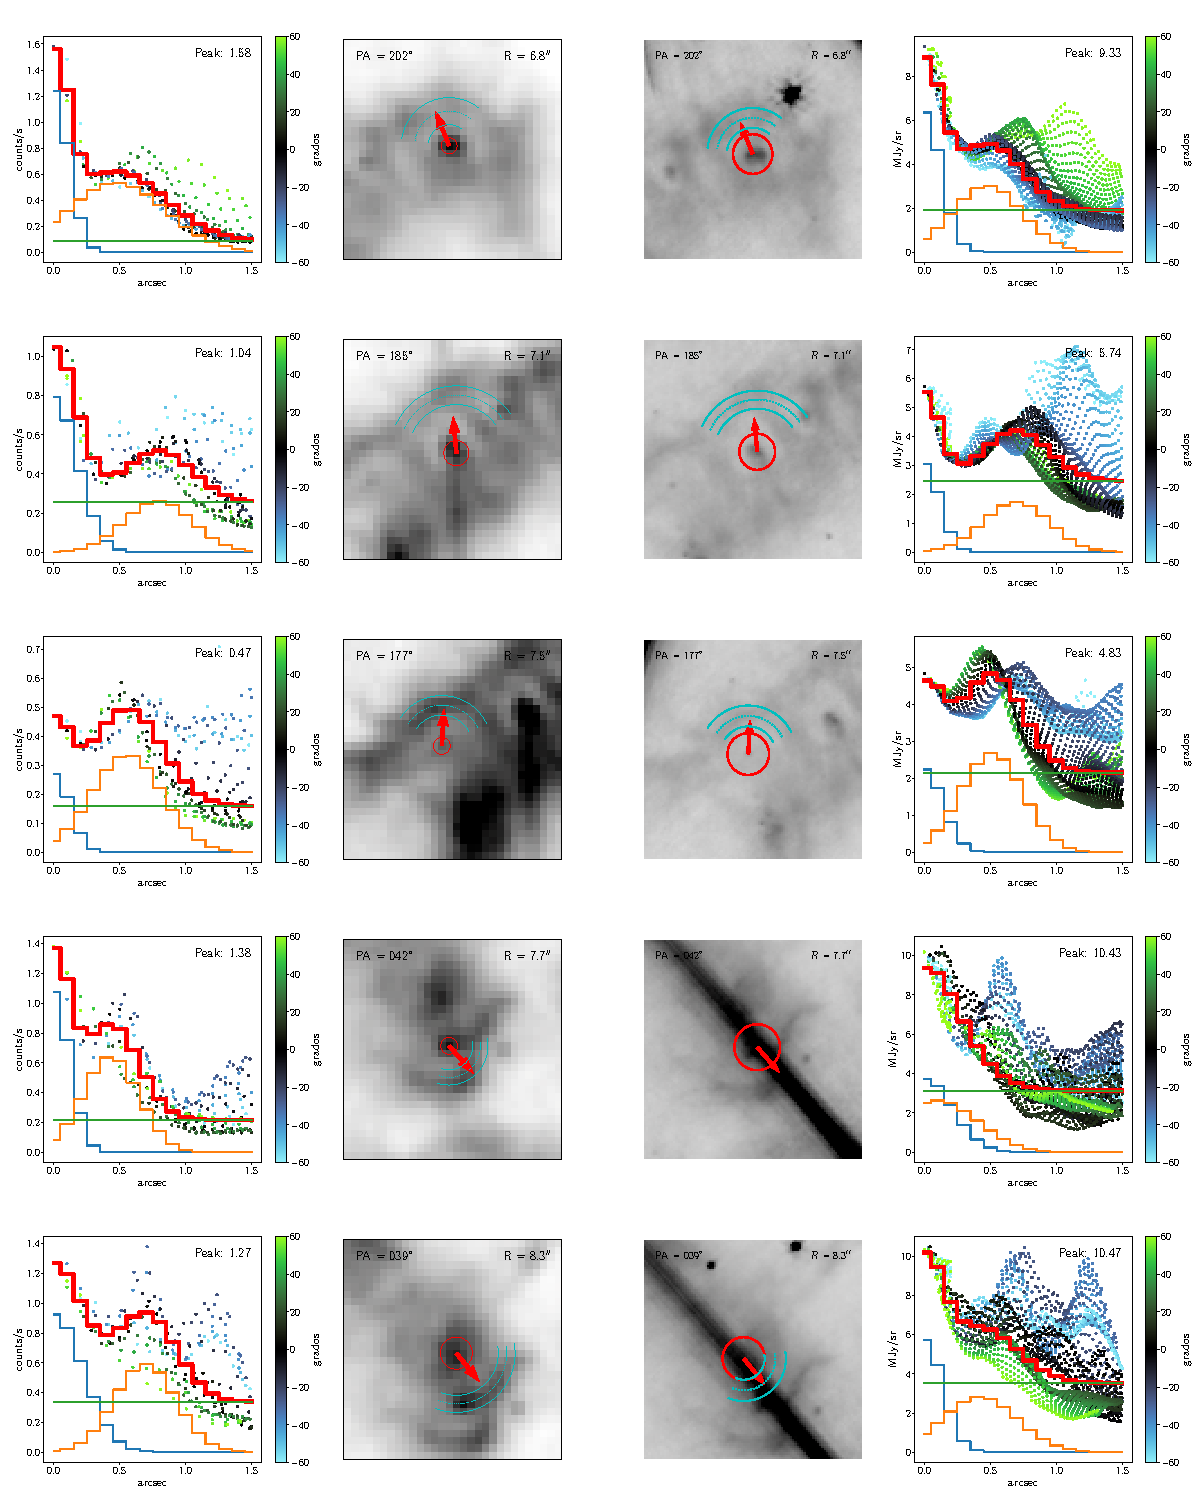
\includegraphics[width=7.5in]{Nuevas imagenes finales/Aj_02.pdf}
  };
\end{tikzpicture}

\newpage

\begin{tikzpicture}[overlay, remember picture]
  % La imagen se coloca en una posición específica
  \node[anchor=south west, xshift=1.3cm, yshift=.2cm] at (current page.south west) {
    \includegraphics[width=7.5in]{Nuevas imagenes finales/Aj_03.pdf}
  };
\end{tikzpicture}

\newpage

\begin{tikzpicture}[overlay, remember picture]
  % La imagen se coloca en una posición específica
  \node[anchor=south west, xshift=1.3cm, yshift=.2cm] at (current page.south west) {
    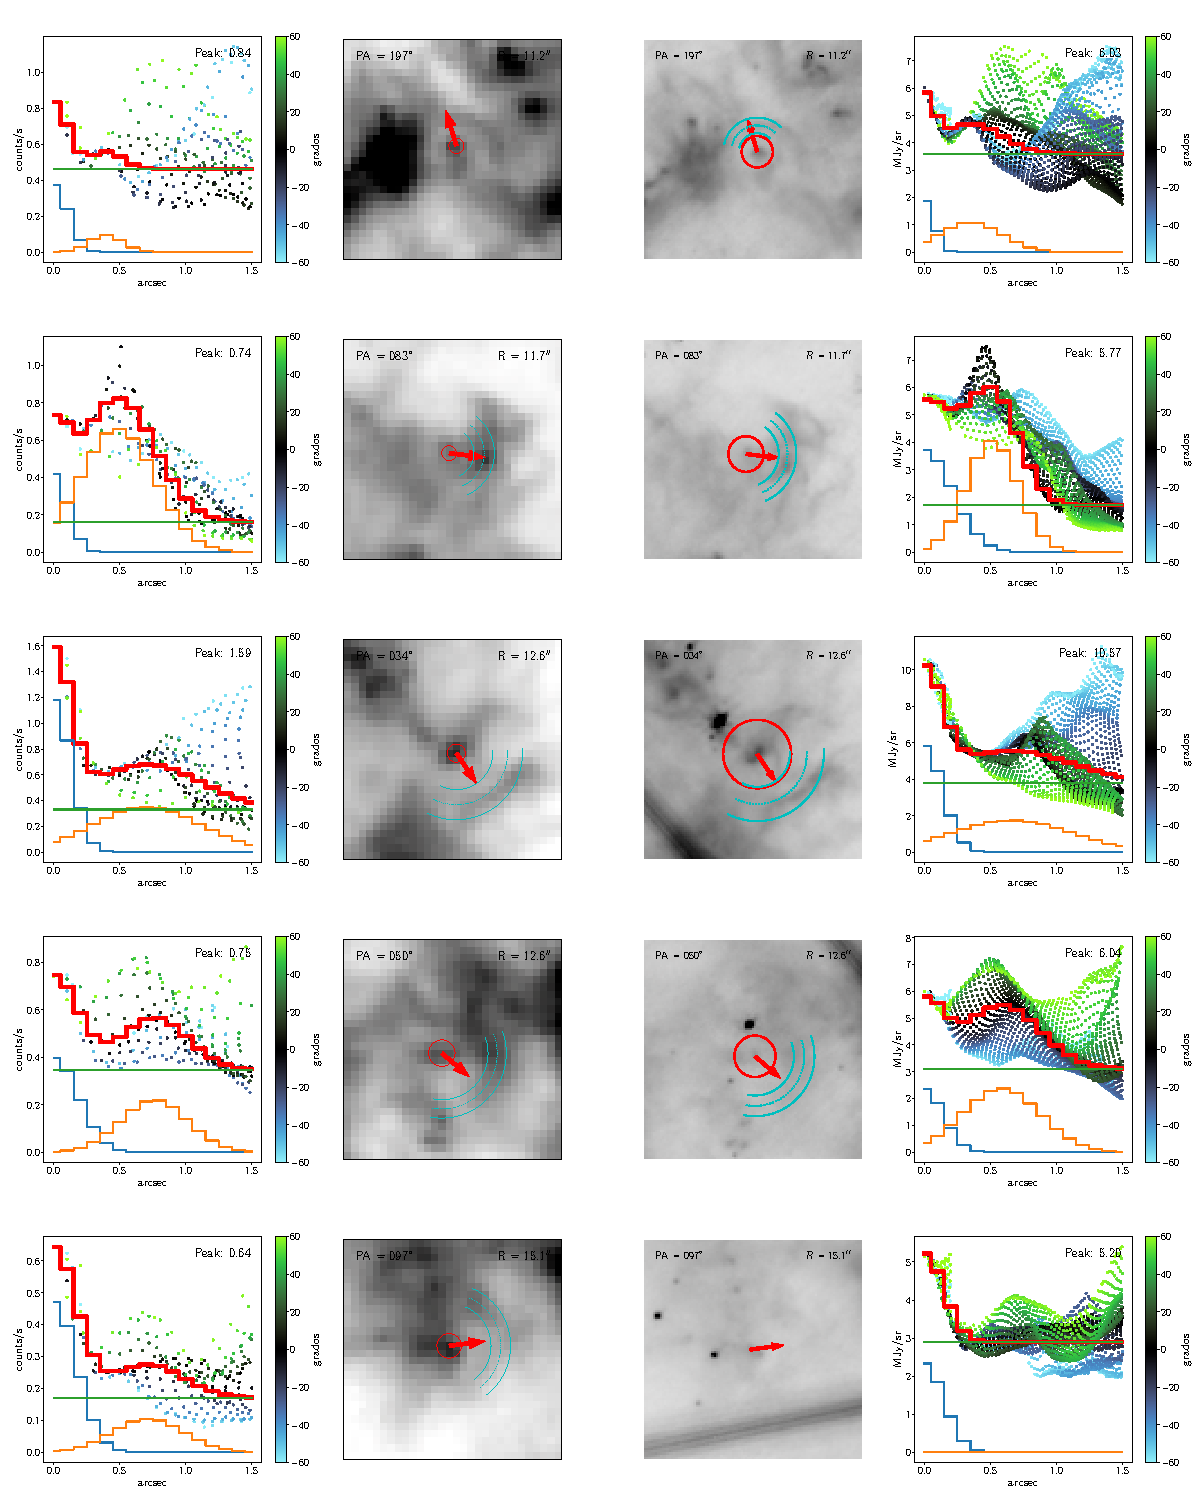
\includegraphics[width=7.5in]{Nuevas imagenes finales/Aj_04.pdf}
  };
\end{tikzpicture}

\newpage

\begin{tikzpicture}[overlay, remember picture]
  % La imagen se coloca en una posición específica
  \node[anchor=south west, xshift=1.3cm, yshift=.2cm] at (current page.south west) {
    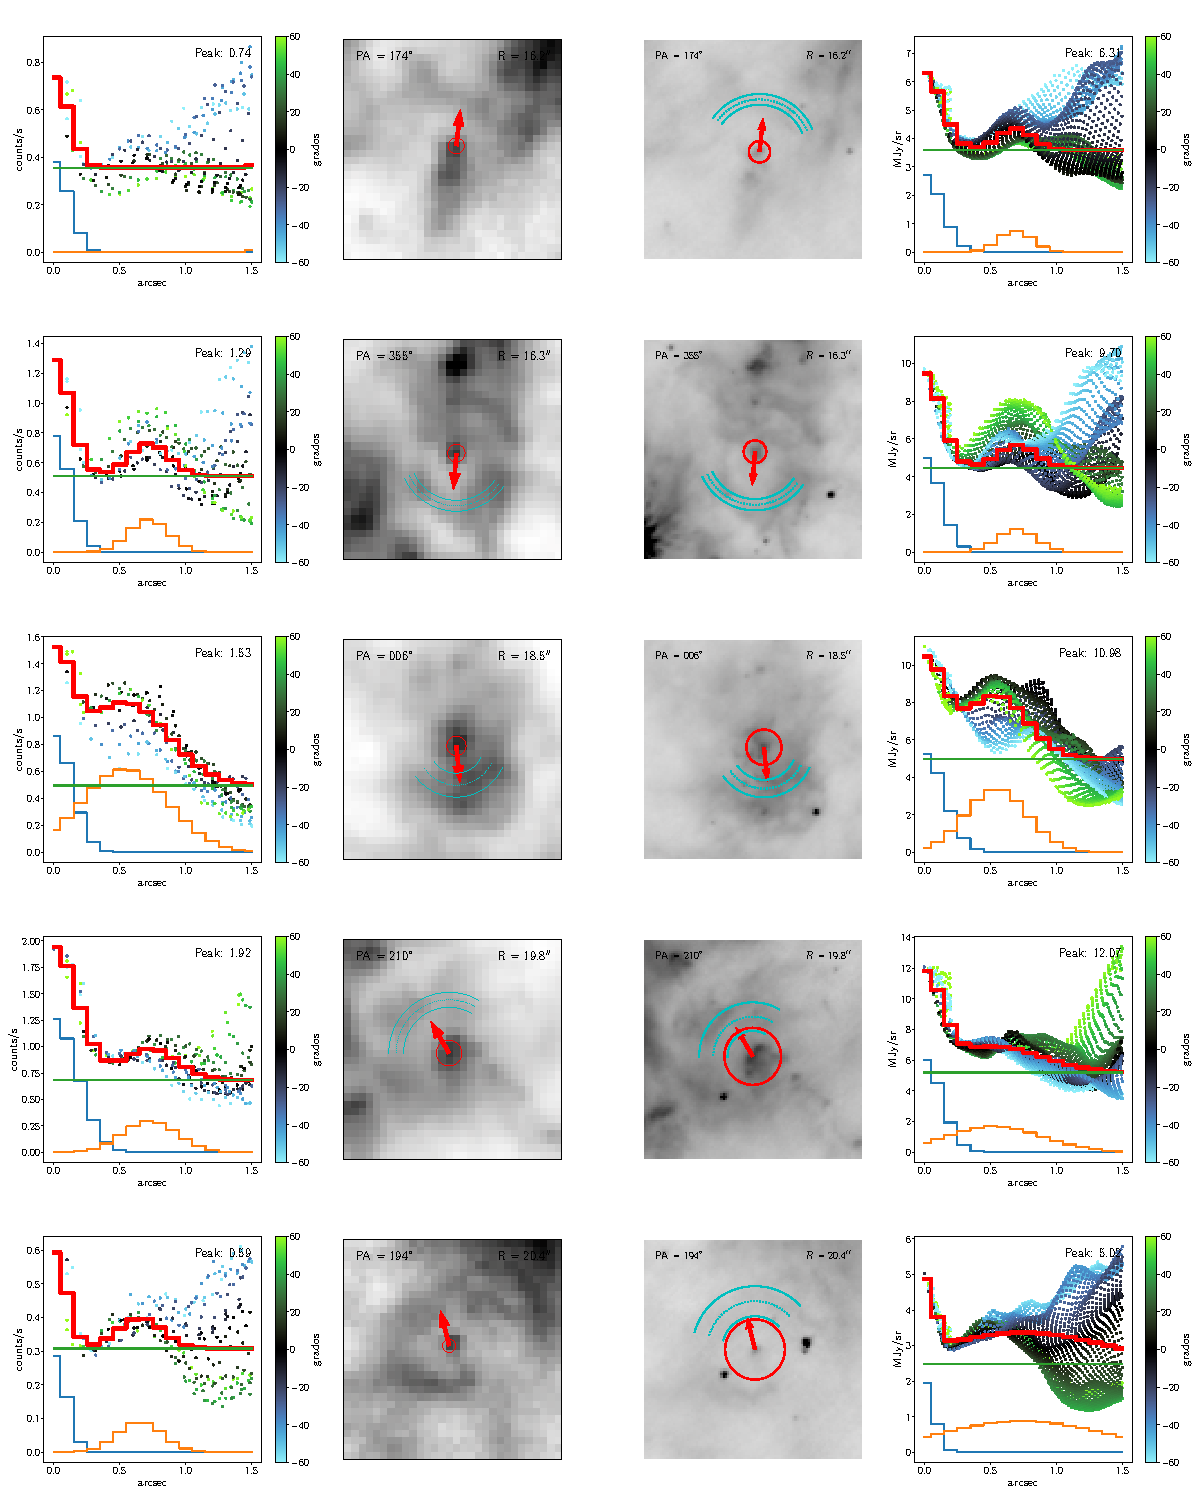
\includegraphics[width=7.5in]{Nuevas imagenes finales/Aj_05.pdf}
  };
\end{tikzpicture}

\newpage

\begin{tikzpicture}[overlay, remember picture]
  % La imagen se coloca en una posición específica
  \node[anchor=south west, xshift=1.3cm, yshift=.2cm] at (current page.south west) {
    \includegraphics[width=7.5in]{Nuevas imagenes finales/Aj_06.pdf}
  };
\end{tikzpicture}

\newpage

\begin{tikzpicture}[overlay, remember picture]
  % La imagen se coloca en una posición específica
  \node[anchor=south west, xshift=.5cm, yshift=5cm] at (current page.south west) {
    \includegraphics{Nuevas imagenes finales/Aj_07.pdf}
  };
\end{tikzpicture}


\bibliography{references}

\end{document}

%%% Local Variables:
%%% mode: LaTeX
%%% TeX-master: t
%%% End:
